\documentclass[12pt]{article}

\usepackage{sbc-template}
\usepackage[utf8]{inputenc}
\usepackage[T1]{fontenc}
\usepackage[brazil]{babel}
\usepackage{graphicx,url}
\usepackage{amsmath,amssymb}
\usepackage{booktabs}
\usepackage{array}
\usepackage{multirow}
\usepackage{xcolor}
\usepackage{tikz}
\usetikzlibrary{positioning,arrows.meta,fit,calc}
\usepackage{enumitem}
\setlist{itemsep=2pt,topsep=4pt}

% Marca visivel para tudo o que ainda depende de resultado ou de informacao do autor.
% Citacao textual: no template SBC as citacoes usam colchetes, "[Autor Ano]".
\providecommand{\citeasnoun}[1]{\cite{#1}}
\newcommand{\pendente}[1]{\textcolor{red}{\textbf{[PENDENTE: #1]}}}

\sloppy

\title{Integração de Aprendizado de Máquina em Redes Quânticas:\\
Controladores Aprendidos e uma Plataforma de Controle Auditável}

\author{Alexandre O. S. Santos\inst{1,2,3}, João M. S. Souza\inst{2,3}, Otto Menegasso Pires\inst{2,3},\\
Leonardo S. Almeida\inst{1}, Gilson Amorim Carvalho\inst{1}}

\address{\inst{1}Centro Universitário Jorge Amado (Unijorge)\\
  Av. Luís Viana Filho, 6775 -- Paralela -- Salvador -- BA -- Brasil
  \nextinstitute
  \inst{2}Quantum Industrial Innovation -- QuIIN\\
  Senai CIMATEC -- Salvador, BA -- Brasil
  \nextinstitute
  \inst{3}Latin America Quantum Computing Center -- LAQCC\\
  Senai CIMATEC -- Salvador, BA -- Brasil}

\email{alexandreoliversan1@gmail.com, joao.marcelo@fieb.org.br,\\
  otto.pires@fieb.org.br, leoalm@gmail.com}

\begin{document}

\maketitle

\begin{abstract}
Operating a quantum network requires continuous decisions: when to purify
entangled pairs, how to compensate polarization drift, how to share a fibre
between classical traffic and key distribution, and how to tune and monitor
key-distribution links. This work develops learned controllers for these
decisions, evaluates them against retuned baselines on held-out seeds, and
integrates them into ORION-Q, a control platform for simulated quantum networks.
The network controllers run on a closed-form physics layer transcribed from the
SeQUeNCe simulator and checked against it to $2.5\times10^{-12}$. On aerial fibre
calibrated to published field statistics, a polarization compensator reaches a
mean QBER of 0.0133 against 0.0461 for a retuned alpha-beta filter (3.5 times,
95\% CI 3.3--3.7), although its weights do not transfer between operating
points; a predictive allocator delivers 2.7 times the classical throughput of
static admission at matched key service; and the routing agent does not beat
the best heuristic. On decoy-state QKD links, an actor-critic agent raises the
provable secret key rate by 8.8--18.9\% over 25--80 km, and a gradient-boosting
classifier over public observables reaches a macro F1 of 0.830 where a QBER
threshold detects one of four attacks; on 515 benign days of the Cambridge
quantum network, that threshold fires on 16.5\% of days. ORION-Q admits all six
components (eleven configurations) through hash-pinned archives without unsafe
deserialization --- the detector, shipped only as a pickle, through an export
rebuilt with the author's pipeline and proven byte-identical to it ---, reproduces
their reference outputs, evaluates them in shadow
mode and exposes an auditable activation flow with review, approval, read-back
and rollback. A preliminary study, in which classical WDM telemetry did not
yield an admission controller better than persistence, motivated this design.
Inside ORION-Q, the five controllers were then run in closed loop on the plant each was
trained on, with the author's packages incorporated into the platform; before
scoring, each campaign regenerates through ORION-Q's replay the author's exported
episodes and published tables. On new seeds, the compensators beat a retuned
alpha-beta filter in every seed at both operating points (3.3 and 4.8 times),
provided the actuator exceeds 120--250~rad/s; the key-rate agent beats the
commissioned setting by 13.6--20.8\% up to 65~km but not at 80~km; the
synchroniser beats the alpha-beta tracker in every run, by up to 5\%; the
allocator carries 2.4--2.6 times the classical traffic of silencing it, at the
same key service; and the routing agent never beats the best heuristic: in
the author's analytic twin it ties it at long deadlines and falls three points
below at the nominal one, and with SeQUeNCe itself as the plant it falls below
at both. On sessions from
random streams the author never used, the detector flags 84--89\% of attack
periods against 7--14\% for the QBER threshold. The author's Verilog, simulated
for the first time, matches its fixed-point references bit for bit. All results
are simulated and no physical actuation is performed.
\end{abstract}

\begin{resumo}
Operar uma rede quântica exige decisões contínuas: quando purificar pares
emaranhados, como compensar a deriva de polarização, como dividir uma fibra entre
tráfego clássico e distribuição de chaves e como ajustar e monitorar enlaces de
QKD. Este trabalho desenvolve controladores aprendidos para essas decisões,
avalia-os contra \textit{baselines} ressintonizados em sementes retidas e os
integra ao ORION-Q, uma plataforma de controle para redes quânticas simuladas.
Os controladores de rede operam sobre uma camada de física em forma fechada
transcrita do simulador SeQUeNCe e conferida contra ele até $2{,}5\times10^{-12}$.
Em fibra aérea calibrada por estatísticas de campo publicadas, um compensador de
polarização atinge QBER média de 0,0133 contra 0,0461 de um filtro alfa-beta
ressintonizado (3,5 vezes; IC 95\% 3,3--3,7), embora seus pesos não se transfiram
entre pontos de operação; um alocador preditivo entrega 2,7 vezes a vazão
clássica da admissão estática a serviço de chave igualado; e o agente de
roteamento não supera a melhor heurística. Em enlaces de QKD com
estados-isca, um agente ator-crítico eleva a taxa de chave secreta provável entre
8,8\% e 18,9\% em vãos de 25 a 80 km, e um classificador por \textit{gradient
boosting} sobre observáveis públicos atinge F1 macro de 0,830, enquanto um limiar
de QBER detecta um de quatro ataques; em 515 dias benignos da rede quântica de
Cambridge, esse limiar dispara em 16,5\% dos dias. O ORION-Q admite os seis
componentes (onze configurações) por meio de pacotes com identidade SHA-256 e sem
desserialização insegura --- o detector, entregue só como \textit{pickle}, por uma
exportação reconstruída com o pipeline do autor e provada idêntica a ele ---, reproduz suas saídas de referência, avalia-os em modo
\textit{shadow} e oferece um fluxo de ativação auditável, com revisão, aprovação,
leitura de confirmação e reversão. Um estudo preliminar, no qual a telemetria
clássica WDM não produziu um controlador de admissão melhor que a persistência,
motivou esse desenho. No ORION-Q, os cinco controladores foram então executados
em laço fechado sobre a planta em que foram treinados, com os pacotes do autor
incorporados à plataforma; antes de pontuar, cada campanha regenera pela réplica
do ORION-Q os episódios exportados e as tabelas publicadas pelo autor. Em
sementes novas, os compensadores venceram um filtro alfa-beta ressintonizado em
todas as sementes nos dois pontos de operação (3,3 e 4,8 vezes), desde que o
atuador ultrapasse 120--250~rad/s; o ator de taxa de chave superou a
configuração de comissionamento em 13,6\% a 20,8\% até 65~km, mas não a 80~km; o
sincronizador venceu o filtro alfa-beta em todas as execuções, por até 5\%; o
alocador carregou 2,4 a 2,6 vezes o tráfego clássico de silenciá-lo, com o mesmo
serviço de chave; e o agente de roteamento não superou a melhor heurística: no
gêmeo analítico do autor, empatou no prazo longo e ficou três pontos abaixo no
nominal, e, com o próprio SeQUeNCe como planta, ficou abaixo nos dois prazos. Em sessões de fluxos
aleatórios que o autor não usou, o detector marcou 84\% a 89\% dos períodos de
ataque, contra 7\% a 14\% do limiar de QBER. O Verilog do autor, simulado pela
primeira vez, é exato ao bit em relação às suas referências em ponto fixo. Todos os
resultados são simulados e nenhuma atuação física é realizada.
\end{resumo}

\noindent\textbf{Palavras-chave:} Redes Quânticas, Aprendizado de Máquina,
Compensação de Polarização, Distribuição Quântica de Chaves, Plano de Controle,
Avaliação Reprodutível.

% =====================================================================
\section{Introdução}

A Internet Quântica pretende distribuir emaranhamento e chaves secretas entre
nós distantes, complementando a infraestrutura clássica de telecomunicações
\cite{kimble2008,wehner2018}. Como fótons sofrem atenuação exponencial na fibra
e o estado quântico não pode ser simplesmente amplificado, o alcance depende de
repetidores quânticos, que combinam geração, armazenamento, purificação e troca
de emaranhamento (\textit{entanglement swapping})
\cite{briegel1998,dur1999,azuma2023}. Na era NISQ (\textit{Noisy
Intermediate-Scale Quantum}), essas operações são imperfeitas e consomem
recursos escassos, como tempo de memória e operações de dois qubits
\cite{preskill2018}.

Operar uma rede desse tipo exige decisões contínuas. Um repetidor precisa
decidir se vale a pena purificar um par cuja fidelidade pode estar abaixo do
limiar útil. Um enlace de distribuição quântica de chaves (QKD) com codificação
em polarização precisa compensar a rotação lenta e aleatória introduzida pela
birrefringência da fibra \cite{xavier2008}. Quando canais clássicos e quânticos
compartilham a mesma fibra, o espalhamento Raman e outras contribuições de ruído
degradam a taxa de erro quântico (QBER) e a taxa de chave secreta (SKR)
\cite{eraerds2010,patel2012,thomas2023}, o que obriga o operador a equilibrar
os dois tipos de tráfego. Para cada uma dessas tarefas já foram propostos
modelos de aprendizado de máquina, por exemplo para roteamento de emaranhamento
por aprendizado por reforço \cite{le2022}.

Um modelo com bom desempenho \textit{offline}, porém, ainda não é um
controlador. Para influenciar decisões de rede, ele precisa de contratos de
entrada e saída explícitos, de comparação com \textit{baselines} simples, como a
persistência (repetir o último valor observado), e de mecanismos que impeçam um
modelo não validado de agir. Sem isso, não é possível distinguir um ganho real de
um artefato do cenário de treino. Este trabalho trata desse problema com a
seguinte pergunta de pesquisa:

\begin{quote}
\textit{Que ganho controladores aprendidos oferecem sobre alternativas simples
nas decisões de controle de uma rede quântica, e como integrá-los a um plano de
controle de forma que cada modelo seja opcional, verificável e comparado a
baselines antes de influenciar decisões?}
\end{quote}

O trabalho começou com uma hipótese mais estreita: a de que a telemetria óptica
clássica de multiplexação por comprimento de onda (WDM) permitiria prever a
fidelidade futura de pares emaranhados e, assim, evitar purificações inúteis.
O estudo preliminar descrito na Seção~\ref{sec:preliminar} testou essa hipótese
com protocolos progressivamente mais rigorosos e encontrou limites claros. Esse
resultado deslocou o foco para dois problemas complementares. O primeiro é
desenvolver controladores aprendidos para decisões específicas e medir cada um
contra a melhor alternativa simples disponível, ressintonizada nas mesmas
condições (Seções~\ref{sec:modelos} a~\ref{sec:qkd}). O segundo é construir uma
plataforma que integre esses controladores sem que nenhum deles possa agir antes
de ser verificado (Seções~\ref{sec:arquitetura} a~\ref{sec:resultados}).

As contribuições são:
\begin{enumerate}  \item uma camada de física para estados Bell-diagonais conferida contra o
        SeQUeNCe e um modelo de fibra calibrado por estatísticas de campo;
  \item controladores aprendidos para compensação de polarização, alocação
        híbrida clássico-quântica, roteamento e temporização de repetidor,
        blocagem de chave, ajuste da taxa de chave, sincronismo e classificação
        de ataques, comparados a \textit{baselines} ressintonizados em sementes
        retidas, com resultados positivos e negativos;
  \item uma validação externa da física de taxa de chave com dados públicos da
        rede quântica de Cambridge;
  \item a arquitetura do ORION-Q, um plano de controle simulado com supervisor
        de segurança independente, trilhas de evidência separadas e diário de
        auditoria;
  \item a admissão de cinco desses componentes (dez configurações) na
        plataforma, com verificação de identidade, leitura segura e paridade
        numérica com as saídas originais, e o bloqueio justificado do sexto;
  \item um fluxo de ativação auditável, com preparação, revisão, aprovação,
        ativação, leitura de confirmação, reversão e recuperação;
  \item uma metodologia de avaliação em três níveis (paridade, \textit{shadow}
        e laço fechado) com protocolo congelado e \textit{baselines}
        obrigatórios;
  \item resultados empíricos, inclusive negativos, registrados de forma
        verificável.
\end{enumerate}

% =====================================================================
\section{Justificativa e Objetivos}

\subsection{Justificativa}

Recursos de um repetidor quântico são escassos: cada tentativa de purificação
consome pares armazenados e tempo de memória, e uma decisão errada não pode ser
desfeita. Ao mesmo tempo, a literatura de aprendizado de máquina para redes
quânticas costuma relatar o desempenho de um modelo isolado, em seu próprio
ambiente de treino. Falta uma camada de engenharia que permita responder, para
cada modelo, três perguntas antes de usá-lo: ele reproduz o comportamento
declarado? Ele supera uma regra simples nas mesmas condições? O que acontece se
ele for ativado e precisar ser revertido? Uma plataforma que torne essas
respostas explícitas reduz o risco de adotar modelos que não agregam valor e
cria uma base reprodutível para comparar novos métodos.

\subsection{Objetivo Geral}

Desenvolver controladores de aprendizado de máquina para decisões de controle
de redes quânticas e uma plataforma de software que os integre a uma rede
simulada de forma opcional, auditável e comparada a \textit{baselines}.

\subsection{Objetivos Específicos}

\begin{itemize}
  \item Construir uma camada de física em forma fechada para estados
        Bell-diagonais, conferida contra o SeQUeNCe, e um modelo de fibra
        calibrado por estatísticas de campo publicadas.
  \item Desenvolver controladores aprendidos para compensação de polarização,
        alocação híbrida, roteamento e temporização, blocagem de chave, ajuste
        da taxa de chave, sincronismo e classificação de ataques, e compará-los
        a \textit{baselines} ressintonizados em sementes retidas.
  \item Confrontar a física de taxa de chave com dados públicos de uma rede de
        QKD implantada.
  \item Formalizar contratos de entrada, saída e ação para funções de controle:
        admissão de purificação, compensação de polarização, sincronização,
        ajuste de taxa de chave, roteamento e alocação de recursos.
  \item Admitir na plataforma os modelos treinados fora dela, com verificação de identidade,
        sem desserialização insegura e com paridade numérica frente às saídas
        de referência.
  \item Implementar um supervisor de segurança independente e um fluxo de
        ativação com revisão, aprovação, ativação, confirmação e reversão.
  \item Avaliar os modelos em modo \textit{shadow} e em laço fechado contra
        persistência e \textit{baselines} clássicos, com protocolo definido
        antes da execução.
  \item Registrar a evidência e os limites de cada modelo em um registro
        verificável.
\end{itemize}

% =====================================================================
\section{Fundamentação Teórica}

\subsection{Repetidores, purificação e troca de emaranhamento}

Um par emaranhado ruidoso pode ser descrito por um estado diagonal na base de
Bell, $\rho=\sum_i c_i\,|\beta_i\rangle\langle\beta_i|$, com populações
$(c_I,c_X,c_Y,c_Z)$ nos quatro estados de Bell; o estado de Werner
\cite{werner1989} é o caso isotrópico, caracterizado apenas pela fidelidade $F$
em relação a $|\Phi^+\rangle$. O protocolo de purificação BBPSSW consome dois
pares de fidelidade $F$ e, com probabilidade de sucesso $p_{\mathrm{suc}}$,
produz um par de fidelidade $F'$ \cite{bennett1996}:
\begin{equation}
F' = \frac{F^2 + \frac{1}{9}(1-F)^2}{p_{\mathrm{suc}}}, \qquad
p_{\mathrm{suc}} = F^2 + \frac{2}{3}F(1-F) + \frac{5}{9}(1-F)^2 .
\label{eq:bbpssw}
\end{equation}
O protocolo só melhora a fidelidade quando $F > 1/2$; abaixo disso, a tentativa
consome recursos sem benefício. O protocolo DEJMPS \cite{deutsch1996} preserva a
estrutura Bell-diagonal completa, em vez de devolver um estado de Werner. A
troca de emaranhamento entre dois pares de Werner com fidelidades $F_1$ e $F_2$
produz
\begin{equation}
F_{\mathrm{out}} = F_1F_2 + \frac{(1-F_1)(1-F_2)}{3},
\label{eq:swap}
\end{equation}
de modo que a fidelidade decai rapidamente ao longo de vários saltos
\cite{briegel1998,dur1999}. Enquanto aguardam, os qubits armazenados sofrem
relaxação de amplitude e de fase, caracterizadas pelos tempos $T_1$ e $T_2$
\cite{nielsen2010}.

\subsection{QKD com estados-isca}

No protocolo BB84 \cite{bennett1984}, transmissores práticos usam laser
atenuado, cujo número de fótons por pulso segue uma distribuição de Poisson.
Pulsos com dois ou mais fótons permitem o ataque de separação por número de
fótons (PNS), que não altera a taxa de erro \cite{brassard2000}. Os
estados-isca \cite{hwang2003,lo2005,ma2005} resolvem esse problema: o
transmissor varia a intensidade ao acaso e, como o espião não sabe qual
intensidade foi usada, os rendimentos por número de fótons $Y_n$ passam a ser
propriedade do canal. Seja $Y_n$ a probabilidade de clique dado um pulso de $n$
fótons e $e_n$ a probabilidade de esse clique estar errado. O ganho e o erro
observados na intensidade $\mu$ são
\begin{equation}
Q_\mu=\sum_{n=0}^{\infty}\frac{\mu^n e^{-\mu}}{n!}\,Y_n,\qquad
E_\mu Q_\mu=\sum_{n=0}^{\infty}\frac{\mu^n e^{-\mu}}{n!}\,Y_n e_n .
\label{eq:ganho}
\end{equation}
Com o protocolo de vácuo mais isca fraca ($\nu<\mu$), obtêm-se o limite
inferior do rendimento de fóton único e o limite superior do seu erro
\cite{ma2005}:
\begin{gather}
Y_1\ge Y_1^L=\frac{\mu}{\mu\nu-\nu^2}\left(Q_\nu e^{\nu}-Q_\mu e^{\mu}\frac{\nu^2}{\mu^2}-\frac{\mu^2-\nu^2}{\mu^2}Y_0\right),\nonumber\\
e_1\le e_1^U=\frac{E_\nu Q_\nu e^{\nu}-e_0Y_0}{Y_1^L\,\nu},
\label{eq:isca}
\end{gather}
e a taxa de chave secreta segue a formulação GLLP \cite{gottesman2004}:
\begin{equation}
R\ \ge\ q\left[Q_1^L\bigl(1-h(e_1^U)\bigr)-f\,Q_\mu\,h(E_\mu)\right],\qquad Q_1^L=Y_1^L\,\mu\,e^{-\mu},
\label{eq:gllp}
\end{equation}
em que $h(\cdot)$ é a entropia binária, $f$ a ineficiência da reconciliação e
$q$ o fator de peneiramento.

Quando sinais clássicos de alta potência compartilham a fibra, fótons gerados
por espalhamento Raman caem na banda do canal quântico, elevam a QBER e reduzem
a taxa de chave \cite{eraerds2010,patel2012,kumar2015}. O projeto do plano
espectral e da potência clássica é, portanto, um compromisso entre os dois
serviços \cite{thomas2023}.

\subsection{Chave secreta com bloco finito}
\label{sec:finita}

Com blocos finitos, a chave extraível é dada por um limite composável
\cite{tomamichel2012}. Para $n$ bits reservados à chave e $k$ bits usados
na estimativa do erro $e$,
\begin{gather}
\ell\le n\left[1-h(e+\mu_k)\right]-\mathrm{leak}_{EC}-\log_2\frac{2}{\varepsilon_{\mathrm{cor}}}-2\log_2\frac{1}{2\varepsilon_{\mathrm{sec}}},\nonumber\\
\mu_k=\sqrt{\frac{(n+k)(k+1)}{nk^2}\ln\frac{1}{\varepsilon_{\mathrm{sec}}}},
\label{eq:finita}
\end{gather}
A fração de teste precisa ser otimizada: fixá-la em 10\% faz o limite convergir
para 90\% da taxa assintótica, e não para ela. Uma consequência da
Eq.~\ref{eq:finita} será usada adiante: a chave de um bloco depende apenas do
número de bits e da sua taxa média de erro. Um trecho ruim envenena todos os
bits que dividem o bloco com ele, e a chave não depende da ordem em que os bits
chegaram. A Eq.~\ref{eq:finita} supõe fonte de fóton único; com pulsos
coerentes de intensidade $\mu$, apenas a fração $\approx e^{-\mu}$ dos bits vem
de um único fóton, enquanto a correção de erros é paga sobre o bloco inteiro
\cite{gottesman2004,lim2014}.

\subsection{Deriva de polarização}

Em QKD com codificação em polarização, a birrefringência da fibra varia com a
temperatura e com vibrações, rotacionando o estado de polarização. Essa rotação
pode ser representada por uma matriz $R(t)\in SO(3)$ que atua no vetor de Stokes
na esfera de Poincaré. Se o estado recebido estiver desalinhado de um ângulo
$\theta$ em relação à base de medição, a probabilidade de erro de projeção é
\begin{equation}
e(\theta) = \sin^2(\theta/2),
\label{eq:erro_pol}
\end{equation}
que se soma à QBER. Sistemas práticos compensam $R(t)$ com controle ativo
\cite{xavier2008}, tipicamente por uma cascata de retardadores com reset sem fim
\cite{noe1988}. Um preditor da rotação futura pode antecipar essa compensação.

\subsection{Modelos e baselines}

Os controladores usam regressão Ridge \cite{hoerl1970}, perceptrons
multicamadas (MLP), redes LSTM \cite{hochreiter1997}, aprendizado por reforço
ator-crítico com estimativa generalizada de vantagem
\cite{sutton2018,mnih2016,schulman2016}, \textit{random forests}
\cite{breiman2001} e \textit{gradient boosting} \cite{friedman2001}. Em séries
temporais com forte autocorrelação, a persistência ($\hat{x}_{t+h}=x_t$) é um
\textit{baseline} difícil de superar; por isso, todo modelo é comparado a ela e
a pelo menos uma regra clássica adicional, ressintonizada nas mesmas condições.
As comparações entre vários candidatos usam correção de Holm \cite{holm1979};
equivalência é testada pelo procedimento TOST \cite{schuirmann1987}; e
proporções usam intervalos de Wilson \cite{wilson1927}.

% =====================================================================
\section{Trabalhos Relacionados}

\subsection{Simuladores e arquitetura}

Simuladores de eventos discretos, como o SeQUeNCe \cite{wu2021} e o NetSquid
\cite{coopmans2021}, modelam componentes físicos, protocolos e pilhas de rede
quântica com alto nível de detalhe. Eles são a base usual para treinar e testar
políticas de controle, mas não tratam da governança de modelos aprendidos
dentro de um plano de controle: verificação de identidade dos pesos,
comparação obrigatória com \textit{baselines}, ativação reversível e auditoria.
A RFC~9340 \cite{kozlowski2023} descreve princípios arquiteturais para uma
Internet Quântica, incluindo a separação entre plano de dados e de controle e o
papel da sinalização clássica; o documento é informativo, e não uma
especificação normativa.

\subsection{Aprendizado aplicado a repetidores e roteamento}

\citeasnoun{wallnofer2020} mostraram um agente de aprendizado por reforço
redescobrindo teleportação, purificação e esquemas de repetidor por simulação.
Para roteamento, o aprendizado por reforço já foi aplicado à escolha de rotas
em redes de comunicação quântica \cite{roik2024} e ao roteamento de
emaranhamento \cite{le2022}. Para destilação, circuitos de purificação foram
otimizados por algoritmo genético \cite{krastanov2019} e por circuitos
parametrizados sob comunicação clássica ruidosa \cite{chittoor2023}. O agente
da Seção~\ref{sec:roteamento} difere desses trabalhos em dois pontos: seu
espaço de ações inclui esperar e descartar, de modo que a política pode escolher
não agir, e o custo temporal de cada primitiva é medido contra o protocolo do
simulador, e não herdado do modelo analítico.

\subsection{Compensação de polarização e estatística de campo}
\label{sec:campo}

O controle de polarização sem fim por cascata de retardadores é um resultado
clássico \cite{noe1988} e continua sendo a base do \textit{hardware} de
compensação. A literatura recente de controle em tempo real é dominada por
otimização clássica: \citeasnoun{young2026} comparam descida de gradiente,
descida por coordenadas, recozimento simulado e algoritmos genéticos para
controle eletrônico de polarização em QKD. Onde aprendizado aparece em enlaces
implantados, costuma tratar da deriva de referencial, como a rede recorrente de
\citeasnoun{zhang2021}; as oportunidades de aprendizado em sensoriamento de
polarização são revisadas por \citeasnoun{rode2025}. Por isso, o compensador da
Seção~\ref{sec:compensador} é comparado a um filtro clássico ressintonizado, e
não a outro modelo aprendido.

Não existe conjunto público de séries temporais de polarização em fibra
terrestre instalada. As melhores caracterizações publicam estatísticas:
\citeasnoun{peterson2004} mediram polarimetria de Stokes a 4~kHz em 220~km de
cabo para-raios óptico, com um tom forte na frequência da rede elétrica e
harmônicos em 120 e 180~Hz; \citeasnoun{ramaswamy2026} caracterizaram 15~km de
cabo aéreo e enterrado ao longo de 11 meses, com densidade espectral de deriva
do tipo \textit{flicker} de expoente $\beta=1{,}0\pm0{,}2$;
\citeasnoun{shi2026} distribuíram emaranhamento por 62~km de fibra
majoritariamente aérea, com polarização estável à noite e movendo-se dezenas de
graus em segundos durante o dia; e \citeasnoun{czegledi2016} fixaram a escala da
deriva lenta em fibra enterrada. O modelo de fibra da Seção~\ref{sec:fibra} é
parametrizado por essas estatísticas.

\subsection{Coexistência clássico-quântica}

Sinais clássicos intensos na mesma fibra injetam ruído por espalhamento Raman
espontâneo \cite{kumar2015}. Os limites de multiplexação em redes
reconfiguráveis foram estudados por \citeasnoun{peters2009} e
\citeasnoun{chapuran2009}, e a operação conjunta com criptografia clássica de
1~Gbit/s por \citeasnoun{eraerds2010}. Em operação metropolitana contínua,
\citeasnoun{dynes2019} relataram 580 dias de três enlaces na rede quântica de
Cambridge, com QBER entre 2,4\% e 2,7\% e um incremento atribuível a um canal
DWDM de 100~Gbit/s. Esses dados públicos são usados na
Seção~\ref{sec:cambridge}.

\subsection{Aprendizado de máquina em QKD}

\citeasnoun{wang2019} mostraram que uma rede neural rasa prevê os parâmetros
ótimos de protocolos com estados-isca a partir dos parâmetros do enlace; o
agente da Seção~\ref{sec:taxa} remove a hipótese de canal conhecido e trata a
escolha como controle sob observação parcial. Na detecção de ataques,
\citeasnoun{mao2020} e \citeasnoun{xu2024} relatam acurácias acima de 95\%, mas
com classes balanceadas e ataques de intensidade fixa, sem reportar alarmes
falsos por hora ou precisão sob prior realista. Ataques de implementação, como
o cegamento de detectores \cite{lydersen2010} e o deslocamento temporal
\cite{zhao2008}, produzem chave aparentemente segura sem alterar a taxa de
erro, o que motiva um monitor capaz de distinguir ataque de falha.

\subsection{Chave finita e fronteira de bloco}

O trabalho mais próximo da blocagem de chave da Seção~\ref{sec:blocagem} é a
prova de segurança de QKD de comprimento variável \cite{tupkary2024}, na qual o
protocolo decide quanta chave extrair a partir dos dados observados. A pergunta
tratada aqui é complementar: não quanto extrair de um bloco dado, mas quais
janelas de tempo formam o bloco.

Na literatura consultada, não identificamos trabalhos que integrem
controladores de diferentes funções em um mesmo plano de controle com admissão
verificável, avaliação \textit{shadow}, comparação obrigatória com persistência
e ativação auditável; essa é a lacuna explorada pela plataforma das
Seções~\ref{sec:arquitetura} a~\ref{sec:resultados}.

% =====================================================================
\section{Estudo Preliminar: Admissão Preditiva com Telemetria WDM}
\label{sec:preliminar}

\subsection{Hipótese e formulação}

A hipótese inicial foi que parâmetros ópticos clássicos observáveis sem medir o
estado quântico (deriva de fase, potência, OSNR, BER, perda e latência) estariam
causalmente acima dos processos de decoerência e, portanto, permitiriam prever a
fidelidade futura $F(t+\Delta t)$ de um par e evitar purificações destinadas a
falhar. A formulação original propôs uma métrica de vida útil de coerência
restante; nos experimentos, porém, o alvo efetivamente estimado foi
$F(t+\Delta t)$ e a decisão avaliada foi a admissão da purificação.

Para penalizar mais a admissão de um par cuja fidelidade real está abaixo do
limiar (falso positivo, FP) do que o descarte de um par útil, usou-se uma perda
quadrática sensível ao custo (CS-MSE):
\begin{equation}
L_{CS} = \frac{1}{N}\sum_{i=1}^{N}\left(F_i-\hat{F}_i\right)^2
\left[1+\lambda\,\mathbb{I}(\mathrm{FP}_i)\right],
\label{eq:csmse}
\end{equation}
em que $\mathbb{I}(\mathrm{FP}_i)$ vale 1 quando a previsão admite um par com
fidelidade real abaixo do limiar. O indicador atua apenas como peso do erro
quadrático, que permanece diferenciável.

\subsection{Fase 1: ruído sintético}

Na primeira fase, a deriva de fase do canal foi gerada por um processo de
Ornstein-Uhlenbeck \cite{uhlenbeck1930}, que é gaussiano e markoviano, e uma
rede EdgeLSTM foi treinada com a perda da Eq.~\ref{eq:csmse} para diferentes
valores de $\lambda$, com dez sementes. A Tabela~\ref{tab:lambda} e a
Figura~\ref{fig:lambda} mostram o compromisso resultante.

\begin{table}[ht]
\centering
\caption{Efeito do peso $\lambda$ da CS-MSE sobre as decisões de admissão
(média $\pm$ desvio-padrão, dez sementes). O \textit{baseline} admite todos os
pares.}
\label{tab:lambda}
\footnotesize
\setlength{\tabcolsep}{3pt}
\begin{tabular}{lcccccc}
\toprule
 & Descartes & Tentativas & Rendimento & $\Delta P_{\text{úteis}}$ & FP & MAE \\
\midrule
\textit{Baseline} & 0 & 796 & 26,38\% & -- & 586,0 & -- \\
$\lambda=1$  & $528{,}0\pm176{,}9$ & $268{,}0\pm176{,}9$ & $86{,}2\pm20{,}5\%$ & $-14{,}8\pm8{,}9$ & $72{,}8\pm171{,}4$ & $0{,}095\pm0{,}053$ \\
$\lambda=5$  & $680{,}3\pm65{,}6$ & $115{,}7\pm65{,}6$ & $90{,}9\pm10{,}7\%$ & $-102{,}8\pm62{,}7$ & $8{,}5\pm10{,}5$ & $0{,}170\pm0{,}010$ \\
$\lambda=10$ & $738{,}3\pm51{,}7$ & $57{,}7\pm51{,}7$ & $90{,}1\pm17{,}0\%$ & $-153{,}9\pm53{,}0$ & $1{,}6\pm3{,}1$ & $0{,}175\pm0{,}003$ \\
$\lambda=20$ & $756{,}1\pm33{,}6$ & $39{,}9\pm33{,}6$ & $100{,}0\pm0{,}0\%$ & $-170{,}1\pm33{,}6$ & $0{,}0\pm0{,}0$ & $0{,}175\pm0{,}004$ \\
\bottomrule
\end{tabular}
\end{table}

\begin{figure}[ht]
\centering
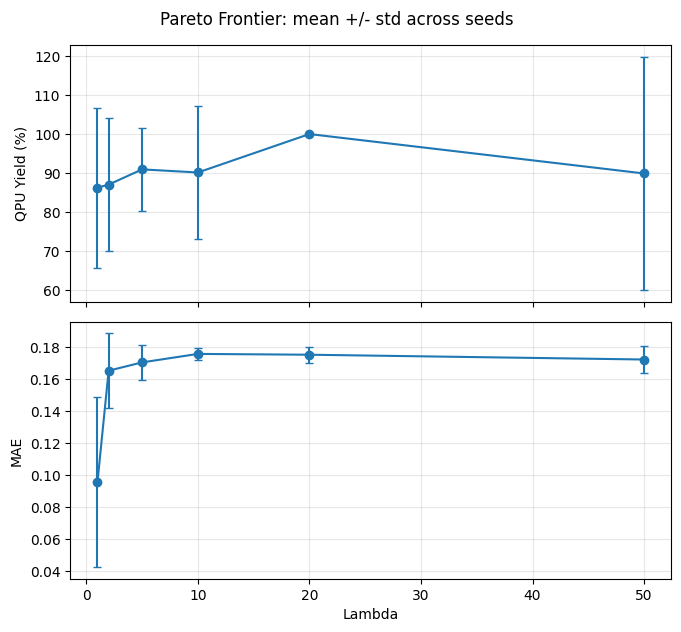
\includegraphics[width=0.62\textwidth]{figuras/fase1_pareto_lambda.png}
\caption{Rendimento da QPU (acima) e MAE (abaixo) em função de $\lambda$; as
barras indicam o desvio-padrão entre dez sementes.}
\label{fig:lambda}
\end{figure}

Com $\lambda=10$, os falsos positivos caem de 586 para $1{,}6\pm3{,}1$, ao custo
de $153{,}9\pm53{,}0$ pares úteis a menos e de um MAE maior, pois a perda
desloca as previsões para baixo de propósito. O rendimento (pares úteis por
tentativa) sobe porque o controlador tenta muito menos; sozinho, esse indicador
favorece políticas que quase nunca agem. A escolha de $\lambda$ depende,
portanto, do custo relativo entre um falso positivo e um par perdido. Em uma
comparação adicional com média móvel, LSTM com MSE, XGBoost e Random Forest, a
EdgeLSTM com CS-MSE teve o menor número de falsos positivos e o menor custo
físico ponderado, enquanto a média móvel teve o maior escore de decisão linear.
Como o custo ponderado atribui peso 100 aos falsos positivos, esse ordenamento
reflete a escolha dos pesos, e não uma superioridade geral do modelo.

\subsection{Fase 2: canal causal e topologia multi-salto}

Na segunda fase, a telemetria passou a derivar dos mesmos parâmetros físicos
que degradam o par (distância, perda, eficiência de transmissão, BER, $T_1$ e
$T_2$), e a fidelidade foi extraída de uma simulação de matriz densidade no
Qiskit Aer \cite{javadi2024}, com erro despolarizante e amortecimentos de
amplitude e de fase. Um detalhe de implementação foi decisivo: o transpilador
remove portas ociosas por padrão e, com isso, apagava a decoerência simulada; o
nível de otimização foi fixado em zero para preservá-la. Como fótons perdidos
geram rodadas com $F=0$, misturadas a rodadas com fidelidade degradada, a rede
foi dividida em duas saídas (DualHead): a probabilidade de chegada do fóton,
treinada com entropia cruzada binária, e a fidelidade condicionada à chegada,
treinada com a CS-MSE. A troca de emaranhamento foi validada contra a
Eq.~\ref{eq:swap}.

\begin{figure}[ht]
\centering
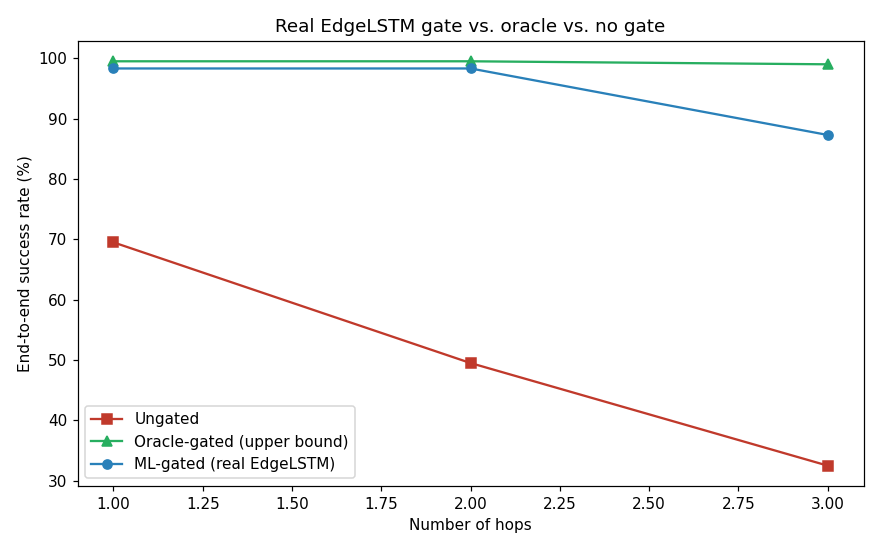
\includegraphics[width=0.62\textwidth]{figuras/fase2_multisalto.png}
\caption{Taxa de sucesso fim a fim entre as tentativas admitidas, para
admissão sem filtro, com filtro EdgeLSTM e com oráculo, em um a três saltos.}
\label{fig:multisalto}
\end{figure}

A Figura~\ref{fig:multisalto} mostra que o filtro por aprendizado de máquina
elevou a taxa de sucesso das tentativas admitidas de 70\% para 98\% em um salto
e de 32\% para 87\% em três saltos, contra 99\% do oráculo. Essa taxa é
condicionada à admissão: ela não mede quantos pares úteis foram entregues, e um
filtro muito conservador pode ter alta taxa de sucesso e baixa vazão. Por isso,
a fase seguinte passou a usar a utilidade líquida por chegada de par como
métrica primária.

\subsection{Reavaliação com protocolo congelado}

Uma primeira campanha com dez sementes indicou rendimento médio de 50,5\%
(IC95\% [46,5; 54,4]) para a DualHead, contra 42,7\% (sem filtro), 43,1\%
(reativo) e 43,0\% (LSTM de saída única), com $p<0{,}001$ após Holm. Essa
comparação, porém, não incluía a persistência nem calibrava a incerteza fora
do conjunto de teste. Um protocolo mais rigoroso foi então definido antes da
execução: ajuste do modelo em um prefixo temporal, calibração da incerteza e dos
limiares em um prefixo posterior, congelamento da política com hash e avaliação
única em dez sementes novas. Duas correções de semântica precederam o teste:
purificação e troca passaram a ser tarefas mutuamente exclusivas, e o limiar
passou a ser o da fidelidade de entrada que produz saída útil pela
Eq.~\ref{eq:bbpssw} (0,625 para uma saída de 0,65).

\begin{table}[ht]
\centering
\caption{Avaliação com protocolo congelado (médias de dez sementes novas).
Utilidade líquida por chegada de par; comparação pareada com persistência e
correção de Holm.}
\label{tab:v526}
\small
\setlength{\tabcolsep}{4pt}
\begin{tabular}{lcccc}
\toprule
Controlador & MAE & Utilidade líquida & Diferença vs. persistência & $p$ (Holm) \\
\midrule
Persistência        & 0,290 & \phantom{$-$}0,067 & -- & -- \\
EdgeLSTM (pontual)  & 0,316 & \phantom{$-$}0,047 & $-0{,}020$ & 1,000 \\
EdgeLSTM (probabilística) & 0,257 & $-0{,}074$ & $-0{,}140$ & 1,000 \\
EdgeLSTM DualHead   & 0,245 & $-0{,}134$ & $-0{,}201$ & 1,000 \\
Oráculo (diagnóstico) & 0,000 & \phantom{$-$}0,364 & -- & -- \\
\bottomrule
\end{tabular}
\end{table}

Nenhuma das três comparações foi positiva e significativa
(Tabela~\ref{tab:v526}); todas as médias favoreceram a persistência. A DualHead
teve o menor MAE entre os modelos neurais, mas a pior utilidade: prever melhor
não se converteu em decidir melhor. A distância até o oráculo mostra que a
informação sobre a fidelidade futura teria valor; o que faltou foi um preditor
que a extraísse de forma útil nesse cenário.

Dados medidos públicos levaram a conclusões compatíveis. Em 65.733 registros
de telemetria óptica de um \textit{testbed} da Scuola Superiore
Sant'Anna\footnote{\url{https://github.com/Network-And-Services/optical-failure-dataset}},
a telemetria WDM passada não melhorou a previsão de OSNR ou BER além do
histórico do próprio alvo em nenhum dos 16 testes. Em varreduras com
equipamento Toshiba publicadas pelo projeto
IrelandQCI\footnote{\url{https://doi.org/10.5281/zenodo.21132088}}, a
coexistência com sinal clássico aumentou a QBER em 0,0132 ($p=0{,}0015$ após
Holm) e reduziu $\log(1+\mathrm{SKR})$ em 0,360 ($p=0{,}011$); a mesma direção
apareceu em dados da Universidade de
Bristol\footnote{\url{https://doi.org/10.5523/bris.61193flfovbn2puknndsr3qm5}}.
Nesses dados, uma regra monotônica baseada somente na potência clássica
ordenou a dominância conjunta QBER--SKR melhor do que uma rede neural de três
saídas (acurácia 0,678 contra 0,563). Nenhuma base pública combinava
telemetria WDM ordenada no tempo com um alvo quântico futuro medido no mesmo
enlace; a hipótese temporal original permanece, portanto, não testada com dados
físicos.

\subsection{Latência de inferência}

A inferência da EdgeLSTM em CPU levou $\tau_{\mathrm{inf}}\approx0{,}5$~ms. Com
o valor $T_2=30~\mu$s adotado na simulação, a razão $\tau_{\mathrm{inf}}/T_2$
fica muito acima de 1: o par se degradaria durante a própria decisão. Como
$T_2$ varia muito entre plataformas de memória \cite{krutyanskiy2023}, essa
conclusão vale para o valor simulado e indica que, para memórias de coerência
curta, a inferência precisaria de \textit{hardware} dedicado.

\subsection{Consequência para o trabalho}

O estudo preliminar mostrou que a qualidade de um modelo só pode ser julgada
contra \textit{baselines} simples, com protocolo congelado e métricas
operacionais, e que métricas isoladas, como rendimento ou MAE, podem enganar.
Em vez de buscar um único preditor melhor, o trabalho passou a construir uma
plataforma na qual qualquer modelo seja submetido a esse tipo de avaliação
antes de influenciar a rede.

% =====================================================================
\section{Substrato Físico e Método dos Controladores}
\label{sec:modelos}

Os controladores das Seções~\ref{sec:rede} e~\ref{sec:qkd} foram
desenvolvidos no pacote qnet\_autopilot, que contém uma camada de física, um
ambiente de decisão, os agentes e os \textit{baselines} atrás de uma mesma
interface, e uma camada de validação. Esta seção descreve o que eles têm em
comum: a física, o modelo de fibra, a física de QKD e as regras de avaliação.

\subsection{Camada de física e conferência com o SeQUeNCe}

Treinar políticas exige milhares de episódios, e um simulador de eventos
discretos completo é lento demais para isso. A camada de física é, por isso,
uma transcrição em forma fechada das rotinas de estados Bell-diagonais do
SeQUeNCe \cite{wu2021}. A transcrição mantém os nomes de variáveis e as
assinaturas do simulador (\texttt{gate\_fid}, \texttt{meas\_fid},
\texttt{p\_succ}, \texttt{c\_I}, \ldots), de modo que as duas implementações
possam ser lidas lado a lado. Sobre ela operam BBPSSW, DEJMPS e a troca de
emaranhamento. A geração é anunciada por um único fóton (\textit{single
heralding}): o formalismo Bell-diagonal não representa a interferência de dois
fótons do esquema de Barrett--Kok \cite{barrett2005}, uma restrição do
formalismo que também torna possível a comparação direta com o simulador.

A transcrição foi conferida em três níveis. No primeiro, cada rotina foi
comparada à chamada correspondente do SeQUeNCe sobre estados aleatórios. No
segundo, trajetórias inteiras foram executadas no ambiente analítico e, em
paralelo, cada par vivo foi reconstruído a partir de objetos do simulador. Em
212 passos sobre duas topologias em cadeia (91 gerações, 22 purificações, 46
trocas e 7 entregas), a maior discrepância em qualquer componente de qualquer
par foi $2{,}5\times10^{-12}$. Dois controles negativos mostram que a
comparação é capaz de falhar: cobrar decoerência de uma ponta do par em vez de
duas, ou usar portas perfeitas, produz divergências acima de $10^{-3}$. No
terceiro nível, a política treinada dirigiu diretamente os protocolos do
simulador sobre as mesmas requisições. Esse confronto também revelou dois
parâmetros que o SeQUeNCe~1.0.0 aceita e ignora em silêncio: a fidelidade de
porta, e o tempo de coerência ajustado depois da construção da memória, pois a
taxa de decoerência só é derivada no construtor. Ambos produzem resultados
otimistas sem levantar erro.

\subsection{Modelo de fibra e pontos de operação}
\label{sec:fibra}

A fibra aplica ao estado de polarização uma rotação $R(t)\in SO(3)$ composta de
três termos: deriva térmica lenta, modelada como processo de Ornstein-Uhlenbeck
\cite{uhlenbeck1930}; uma banda mecânica de tons com harmônicos; e saltos
discretos. O modelo existe em dois pontos de operação. O ponto de
\textit{desenvolvimento} (banda acústica em 40~Hz, deriva de 0,05~rad/s) foi
escolhido por plausibilidade, antes da calibração. O ponto \textit{calibrado}
vem das estatísticas de campo da Seção~\ref{sec:campo}: tom de 60~Hz com harmônicos em 120 e
180~Hz \cite{peterson2004} e deriva de 0,02~rad/s, compatível com o expoente
espectral medido por \citeasnoun{ramaswamy2026}. A recalibração veio depois de
parte dos resultados; por isso, cada resultado indica o ponto em que foi
medido. A comparação principal do compensador foi repetida nos dois.

\subsection{Física de QKD e ataques}
\label{sec:ataques}

A camada de QKD implementa o BB84 com estados-isca pelas
Eqs.~\ref{eq:ganho}--\ref{eq:gllp}, com amostragem binomial de blocos finitos
e três limitações do receptor: tempo morto, pós-pulsos
(\textit{afterpulsing}) e erro intersímbolo por dispersão cromática. Os ataques
são modelados como transformações dos rendimentos $(Y_n,e_n)$, e os observáveis
são recalculados pelo mesmo caminho de código do canal honesto
(Tabela~\ref{tab:ataques}). Assim, o que o receptor observa é derivado da
física, e um ataque sem assinatura física não ganha assinatura no conjunto de
dados. A Figura~\ref{fig:ataques} mostra a consequência: cada ataque deixa uma
assinatura diferente, e o divisor de feixe não deixa nenhuma.

\begin{table}[ht]
\centering
\caption{Ataques modelados como modificações do canal.}
\label{tab:ataques}
\small
\begin{tabular}{>{\raggedright\arraybackslash}p{3.3cm}>{\raggedright\arraybackslash}p{4.9cm}>{\raggedright\arraybackslash}p{4.5cm}}
\toprule
Ataque & Ação sobre o canal & Assinatura \\
\midrule
\textit{Intercept-and-resend} & $e'_n=(1-q)e_n+q\left(\tfrac{1}{2}e_n+\tfrac{1}{4}\right)$ & só o erro; ganho intacto \\
PNS & $Y'_1=(1-b)Y_1$; $Y_{n\ge2}$ compensado & $Q_\mu$ e $E_\mu$ intactos; $Q_\nu$ cai \\
Cegamento de detector & $Y'_{n\ge1}\ge p_{\text{forçado}}$; $Y'_0=Y_0+\ell$ & ganho acima da perda; vácuo clica \\
Divisor de feixe & identidade & nenhuma, por construção \\
\bottomrule
\end{tabular}
\end{table}

\begin{figure}[ht]
\centering
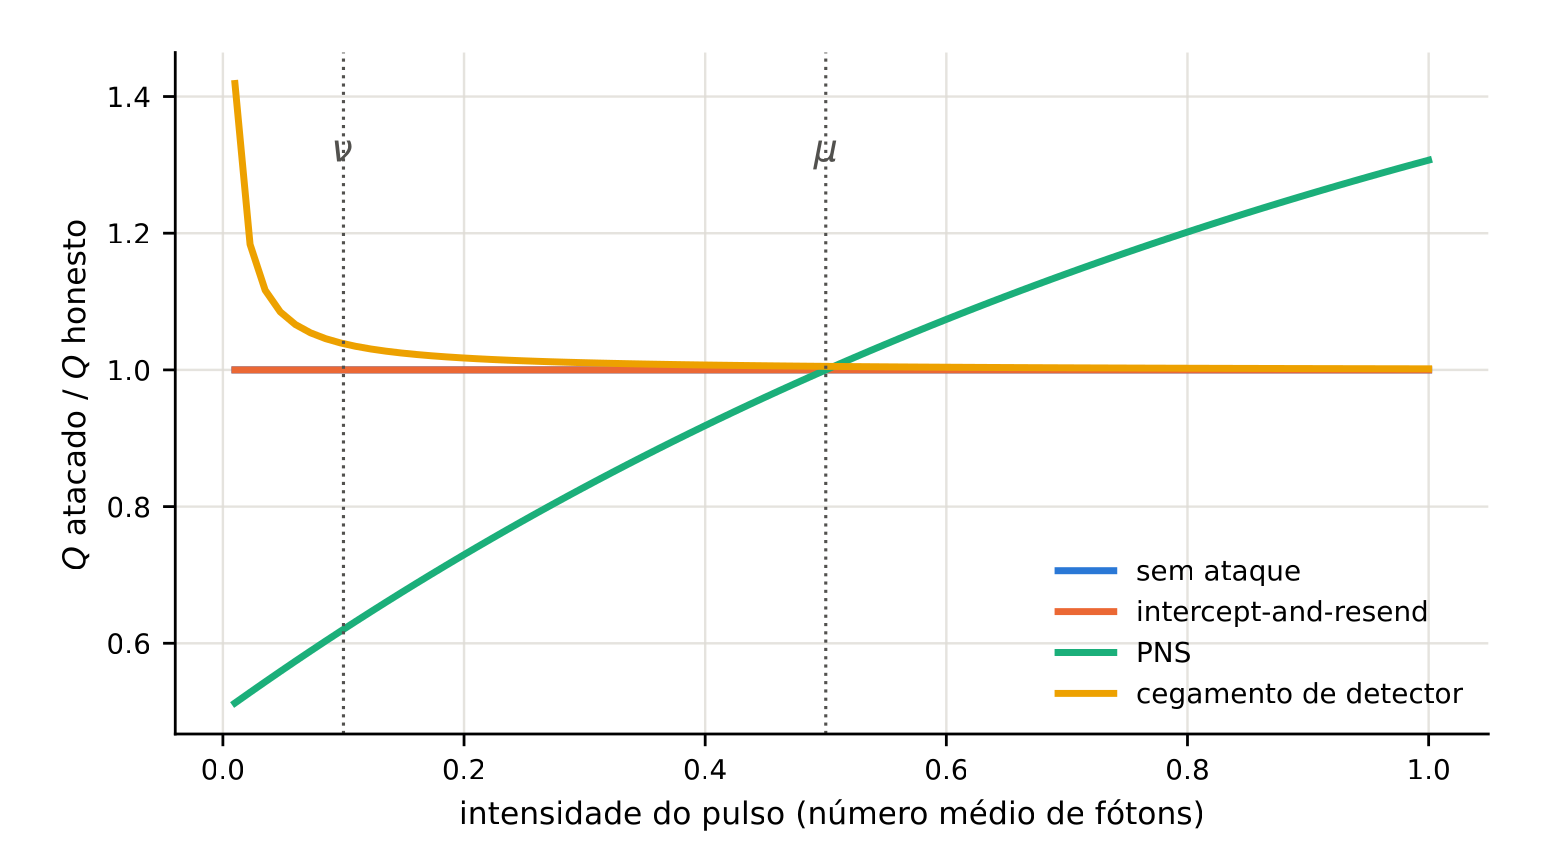
\includegraphics[width=0.8\textwidth]{figuras/qkd_ganho_ataques.png}
\caption{Ganho sob ataque dividido pelo ganho honesto, a 50~km, calculado
diretamente da física. O PNS mantém o ganho na intensidade do sinal ($\mu$) e
não consegue mantê-lo na isca fraca ($\nu$); o \textit{intercept-and-resend}
não altera o ganho; o cegamento empurra o ganho acima do que a perda permite.}
\label{fig:ataques}
\end{figure}

A unidade de simulação é um episódio: um enlace operando por 10 minutos, com
acerto de contas a cada segundo ($10^9$ pulsos por período a 1~GHz), deriva de
polarização abaixo e um evento que começa em instante não anunciado. O primeiro
minuto é livre de eventos e funciona como calibração de comissionamento, e o
vão é sorteado entre 20 e 70~km. Cada ataque sorteia um perfil temporal (degrau,
40\%; rampa, 35\%; intermitente, 25\%), e 40\% dos episódios de ataque carregam
uma excursão térmica simultânea.

\subsection{Regras de avaliação}

Quatro regras valem para todos os controladores. Primeira: nenhum controlador vê
a verdade. O compensador recebe estimativas binomiais obtidas de fótons de
monitoramento, nunca a rotação verdadeira; colunas de verdade ficam num espaço
de nomes próprio, e a construção de janelas levanta erro se uma delas for usada
como característica; o alvo de treino é uma medição futura; e a correção em
vigor em cada instante foi calculada com dados de pelo menos uma latência de
idade. Segunda: todo \textit{baseline} é ressintonizado em cada ponto de
operação, e comparações entre políticas são pareadas por requisição quando a
variância entre tarefas domina. Terceira: sementes de teste são disjuntas das
de treino e de ajuste, a divisão temporal é cronológica com intervalo de guarda,
e a divisão dos dados de ataque é por episódio. Quarta: todo número de destaque
traz intervalo de confiança de 95\% por \textit{bootstrap} sobre sementes
(10.000 reamostragens; 2.000 no alocador, cujas fronteiras são refeitas em cada
uma), e quando o \textit{baseline} é o melhor temporizador escolhido com
retrospectiva, essa escolha é refeita dentro de cada reamostragem. Resultados
negativos são reportados como tais.

% =====================================================================
\section{Controladores de Rede}
\label{sec:rede}

\subsection{Compensação de polarização}
\label{sec:compensador}

O compensador recebe uma janela de estimativas recentes da rotação, expressas
como incrementos relativos ao instante atual, o que torna o problema invariante
a translação na esfera de Poincaré. Ele prevê a rotação uma latência de controle
(40~ms) à frente. Três famílias são comparadas no mesmo laço fechado:
persistência; filtro alfa-beta, ressintonizado por busca em grade em cada ponto
de operação; e preditores ajustados, isto é, regressão Ridge, que é o preditor
de Wiener para um processo gaussiano estacionário, e um MLP. O comando previsto
é convertido em ângulos de uma cascata de retardadores X-Y-X com curso finito,
velocidade finita e reset sem fim \cite{noe1988}, de modo que a avaliação inclui
o custo de mover o atuador.

\begin{table}[ht]
\centering
\caption{Compensação em laço fechado no ponto de desenvolvimento: 8 execuções
de 20~s com sementes retidas e atuador ideal. IC de 95\% por
\textit{bootstrap} entre colchetes. O resíduo é o ângulo de rotação residual.}
\label{tab:comp_dev}
\small
\begin{tabular}{lcccc}
\toprule
Compensador & QBER média & p95 & Disponibilidade & Resíduo (mrad) \\
\midrule
Sem compensação & 0,1316 & 0,3341 & 56,0\% & 857,5 \\
Persistência & 0,1329 [0,128; 0,138] & 0,3253 & 50,1\% & 876,9 \\
Extrapolação linear & 0,3692 & 0,7953 & 17,2\% & 1724,6 \\
Filtro alfa-beta & 0,0383 [0,036; 0,041] & 0,0985 & 96,6\% & 450,8 \\
Ridge (Wiener) & 0,0077 [0,0072; 0,0083] & 0,0211 & 99,9\% & 193,9 \\
MLP & 0,0074 [0,0069; 0,0079] & 0,0203 & 99,9\% & 188,6 \\
\bottomrule
\end{tabular}
\end{table}

A Tabela~\ref{tab:comp_dev} mostra duas linhas que merecem atenção antes das
melhores. A persistência é pior do que não corrigir: com 40~ms de latência, ela
aplica uma correção que a vibração já tornou obsoleta. A extrapolação linear é
pior ainda, porque diferenciar duas estimativas ruidosas dobra a variância.
Compensar mal é uma possibilidade real, e é por isso que o \textit{baseline}
relevante é o alfa-beta ressintonizado. Depois de um salto na fibra, a
recuperação (mediana e percentil 90) leva 0,9 e 52~ms para Ridge e MLP, 11,5 e
73~ms para o alfa-beta e 236 e 473~ms para a persistência; sem compensação,
apenas 3 dos 8 saltos se recuperam antes do fim da execução.

A vantagem do preditor exige um atuador capaz de segui-lo. Variando a velocidade
da cascata de retardadores, o preditor mantém a vantagem acima de 250~rad/s; entre
120 e 250~rad/s os dois empatam; e abaixo de 120~rad/s o filtro clássico vence,
porque um dispositivo lento filtra o comando como um passa-baixas. Em 20~s, o MLP
move os elementos por cerca de 9.300~rad, contra 3.900 do alfa-beta. O MLP empata
com o Ridge em todas as comparações deste ponto, o que é esperado: para um
processo gaussiano estacionário, o preditor ótimo é linear.

\begin{table}[ht]
\centering
\caption{Compensação em laço fechado no ponto calibrado (tom de 60~Hz com
harmônicos em 120 e 180~Hz; deriva de 0,02~rad/s): 6 execuções de 20~s com
sementes retidas. ``Desenvolvimento'' indica o modelo da
Tabela~\ref{tab:comp_dev} transplantado sem retreino.}
\label{tab:comp_cal}
\small
\begin{tabular}{llcc}
\toprule
Compensador & Treinado em & QBER média & IC 95\% \\
\midrule
Sem compensação & -- & 0,0646 & [0,053; 0,078] \\
Persistência & -- & 0,1226 & [0,117; 0,127] \\
Filtro alfa-beta & ressintonizado & 0,0461 & [0,045; 0,047] \\
Ridge (Wiener) & ponto calibrado & 0,0133 & [0,0125; 0,0140] \\
MLP & ponto calibrado & 0,0136 & [0,0128; 0,0144] \\
Ridge (Wiener) & desenvolvimento & 0,2709 & [0,263; 0,278] \\
MLP & desenvolvimento & 0,2594 & [0,253; 0,266] \\
\bottomrule
\end{tabular}
\end{table}

A Tabela~\ref{tab:comp_cal} repete a comparação no ponto calibrado, com os
preditores retreinados ali pela mesma receita e o alfa-beta ressintonizado pela
mesma busca. A vantagem sobrevive: o filtro fica 3,47 vezes acima do Ridge
(IC 95\% 3,28--3,71) e 3,38 vezes acima do MLP (3,18--3,62), contra 5,2 vezes
(4,7--5,8) no ponto de desenvolvimento, e os preditores vencem nas 6 sementes.
Mantidos os ganhos do ponto de desenvolvimento, o filtro teria ficado em 0,0524
e a razão em 3,9; a ressintonia reduz a margem em um oitavo, e é por isso que
ela é feita. Os modelos treinados a 40~Hz e transplantados chegam a
0,26--0,27, quatro vezes pior que não compensar (IC 3,4--5,1). O que se
transfere entre pontos de operação é a receita de treino, não os pesos.

\textbf{Generalização em frequência.} Um compensador por enlace exige um
polarímetro e um treino por enlace. Testou-se, por isso, se um único modelo
cobre a faixa de frequências plausível. Ele não cobre
(Figura~\ref{fig:generalizacao}). Treinado sobre 45--180~Hz e testado em cinco
tons retidos, o modelo ficou em QBER média 0,0615 com janela longa densa e
0,0793 com a janela curta original, ambos piores que o alfa-beta (0,0480) e 2,4 a
3,1 vezes piores que o especialista treinado na frequência certa (0,0252). A
dispersão entre três inicializações foi no máximo 0,0057, quase uma ordem abaixo
das diferenças. Alongar a janela de 32 para 126~ms ajudou (de 0,079 para 0,062),
mas não bastou; fornecer a frequência estimada como entrada piorou as duas
janelas. Só aqui o MLP supera o Ridge: uma mistura de frequências não é um
processo gaussiano estacionário, e o preditor precisa inferir o tom antes de
prever sua fase. A recomendação que sobrevive é uma família de modelos de faixa
estreita com um seletor.

\begin{figure}[ht]
\centering
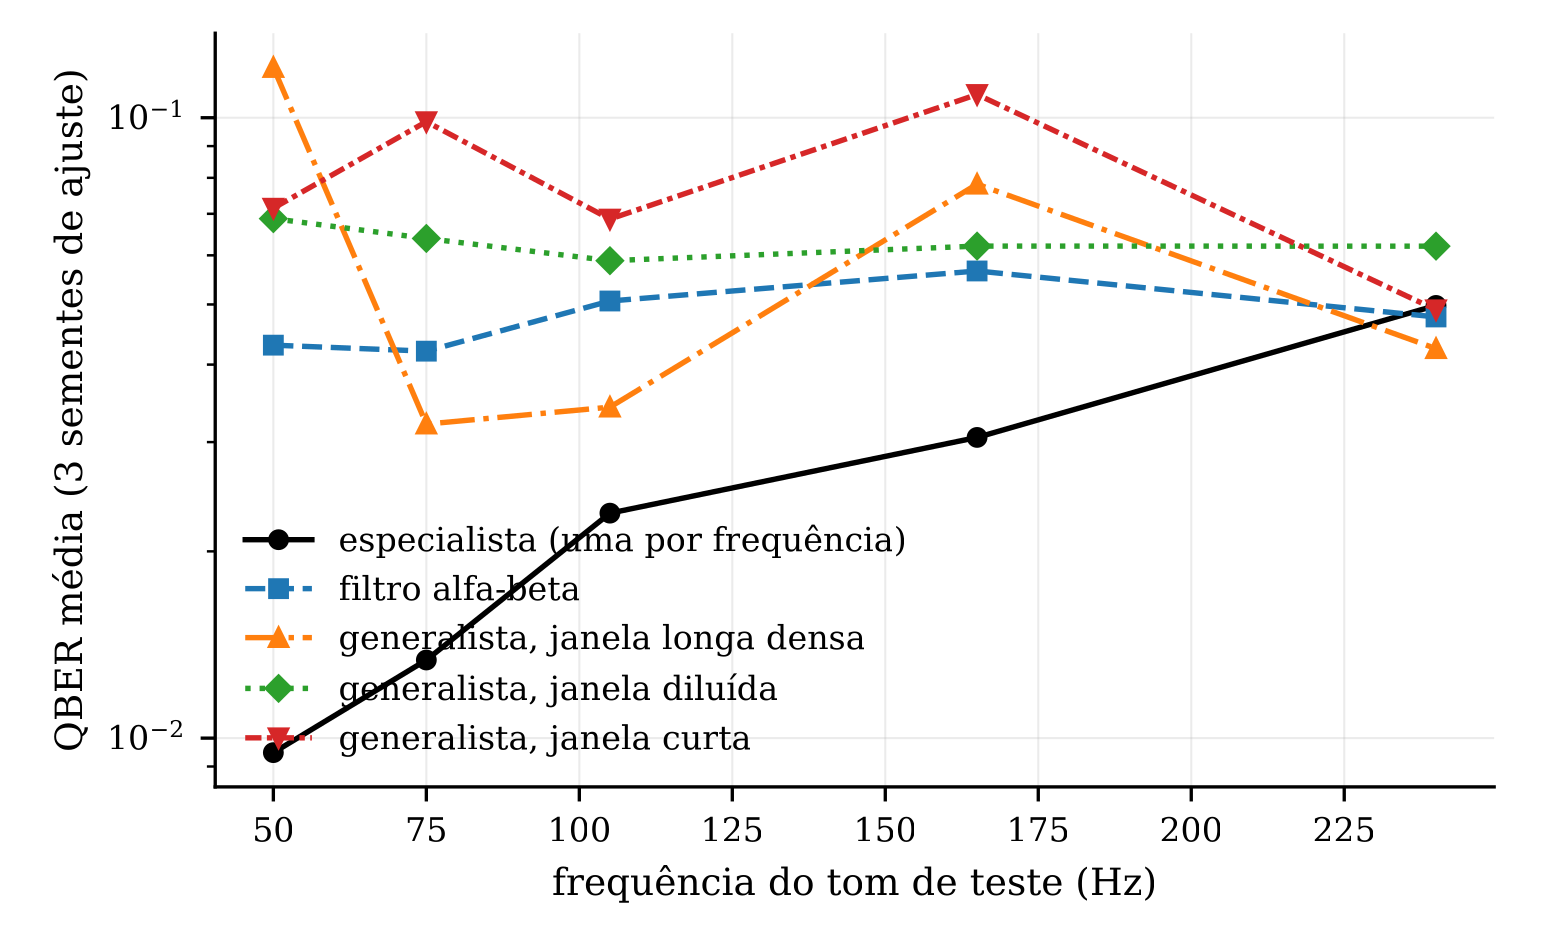
\includegraphics[width=0.85\textwidth]{figuras/comp_generalizacao.png}
\caption{Um modelo único treinado sobre 45--180~Hz, avaliado por tom retido
(QBER média em três sementes de ajuste, escala logarítmica). A janela longa
densa chega perto do especialista em 75 e 105~Hz e falha em 50~Hz; a janela
diluída é plana e medíocre em toda a banda.}
\label{fig:generalizacao}
\end{figure}

\textbf{Porte para ponto fixo.} Um compensador que roda a cada 2~ms perto do
atuador é candidato a lógica programável. Um modelo de referência em ponto
fixo, bit a bit, de todo o caminho de inferência (incluindo logaritmo e
exponencial em SO(3) por CORDIC) foi avaliado no mesmo laço fechado. Dezesseis
bits bastam: o MLP fica em 1,02 e o Ridge em 0,98 vez a QBER do modelo em ponto
flutuante. O limite é um degrau: a 14 bits, 1,05 e 1,28; a 12 bits, os dois vão
a 0,15--0,17, o nível da persistência. A 16 bits, o Ridge requer 144
multiplicações-acumulações por inferência e 0,29~KiB de parâmetros, e um único
multiplicador-acumulador serial a 100~MHz resolve sua parte linear em 1,4~$\mu$s,
contra um período de controle de 2~ms. O código Verilog gerado foi conferido por
um modelo de ciclos em Python, exato ao bit em 64 vetores de referência; a
simulação em ferramenta HDL e a síntese foram feitas depois, no ORION-Q
(Seção~\ref{sec:rtl}), onde o porte também foi avaliado nos dois pontos de
operação (Seção~\ref{sec:quant}).

\subsection{Alocação híbrida clássico-quântica}
\label{sec:alocador}

A alocação é tratada como admissão: a cada instante, que fração da fibra
liberar ao tráfego clássico, sabendo que o ruído Raman induzido eleva a QBER do
canal quântico \cite{kumar2015} e que o serviço de chave é avaliado pela
Eq.~\ref{eq:finita}. As políticas comparadas são admissão estática em vários
níveis, limiar reativo sobre a QBER observada e um alocador preditivo que prevê
a deriva e só admite tráfego clássico quando prevê estabilidade; a deriva usada
é o resíduo deixado pelo compensador do ponto de desenvolvimento.

Cobrar o custo de bloco finito reduz o serviço de chave de todas as políticas
entre 30\% e 55\%, sem alterar a ordenação, mas move o ponto de operação. Por
isso, as fronteiras foram retraçadas em vez de a conclusão ser extrapolada. A
serviço de chave igualado, o alocador preditivo entrega 2,7 vezes a vazão
clássica da admissão estática (IC 95\% 2,6--2,9, com as fronteiras retraçadas
em cada reamostragem), contra 2,4 vezes com chave assintótica. Com os
preditores, blocos de 10~s recuperam 80\% da taxa assintótica; com a
persistência, nenhuma duração recupera mais que 3\%. O ganho vem da lei de
controle frente à admissão estática, e não do componente de previsão: a
documentação do pacote não registra vantagem relevante da previsão Ridge sobre a
persistência.

\subsection{Roteamento e temporização}
\label{sec:roteamento}

Roteamento e temporização de repetidor são formulados como um único processo
de decisão de Markov, com ações \{\textsc{gerar}, \textsc{purificar},
\textsc{trocar}, \textsc{entregar}, \textsc{descartar}, \textsc{esperar}\}. O
estado é descrito por 11 características globais (fração do prazo restante,
progresso da entrega, pares vivos, fidelidades média e máxima, pressão de
memória, cobertura do caminho, limiar da requisição e orçamento consumido), e
cada ação legal por 23 características, entre elas a probabilidade de
\textit{heralding} do enlace, a fidelidade prevista do resultado e a idade do
par mais antigo. A recompensa paga uma entrega qualificada mais um bônus
proporcional à margem de fidelidade, e cobra um custo de tempo proporcional à
fração do prazo consumida e um custo fixo por tentativa de geração. A política
é um ator-crítico com GAE($\lambda$) \cite{schulman2016,mnih2016}, com
retropropagação manual conferida contra diferenças finitas até $10^{-10}$ e
modelagem de recompensa baseada em potencial \cite{ng1999}; a avaliação sempre
reporta a recompensa não modelada.

O primeiro resultado veio da conferência com o simulador. O ambiente analítico
cobrava, por tentativa de \textit{heralding}, uma travessia do vão; o protocolo
do SeQUeNCe cobra 4,1 vezes esse tempo, porque uma tentativa é uma negociação de
várias mensagens, e a razão se mantém ao longo de um fator de oito em distância.
Corrigido o custo, a vantagem de roteamento medida antes desapareceu, e o agente
passou a empatar com as melhores heurísticas nos prazos nominais. Como o
parâmetro estava nos ambientes de treino e de teste, nenhuma avaliação interna
poderia tê-lo revelado.

Com prazos quatro vezes maiores, a política treinada não faz nada: zero
tentativas de geração, zero trocas, até o fim do prazo. A causa é a recompensa,
não o treino: o custo por tentativa é fixo, enquanto o custo de tempo é uma
fração do prazo. O prêmio disponível para qualquer aprendiz (melhor heurística
menos a política de não fazer nada) cai de 0,126 entrega no prazo nominal para
0,040 no prazo quádruplo. Com uma cobrança invariante ao prazo, o prêmio volta a
0,448 e três de três sementes passam a treinar; ainda assim, a melhor semente
fica em $-0{,}012\pm0{,}014$ entrega contra a heurística gulosa, pareado por
requisição: um empate. Nesse regime, a geração domina o orçamento, e tomar a
maior fidelidade disponível já está perto do ótimo. O agente aprendido não é
melhor que a heurística, e é apresentado aqui como resultado negativo.

\subsection{Blocagem de chave}
\label{sec:blocagem}

O controlador de blocagem escolhe as fronteiras dos blocos de amplificação de
privacidade. Ele parte da consequência da Eq.~\ref{eq:finita} apontada na
Seção~\ref{sec:finita}: como a chave de um bloco depende apenas do número de bits e da taxa
média de erro, e não de quando os bits chegaram, janelas boas separadas no tempo
podem ser liquidadas juntas. Três estratégias são comparadas: um temporizador
que corta a cada $T$ segundos; um oráculo por intervalos, que escolhe com
retrospectiva a partição contígua ótima em $O(n^2)$; e um oráculo agrupado, que
abandona a contiguidade ordenando os segmentos por taxa de erro, propriedade
conferida contra força bruta. O controlador causal correspondente vê apenas os
10\% de bits que o protocolo publica para estimar parâmetros e, a cada instante,
compara três continuações: encerrar o bloco, seguir com ele ou pular o
segmento. Não há constante de ajuste na regra.

Em 12 sementes de teste no ponto de desenvolvimento, sobre o enlace compensado
por persistência (QBER 0,134), temporizadores de 5~s ou mais produzem zero bit
em todas as sementes. O controlador entrega 4.075~bit/s (IC 95\% 3.590--4.566),
7,9 vezes o melhor temporizador escolhido com retrospectiva (6,9--9,0) e 95\% do
seu oráculo. Com os melhores compensadores, o melhor bloco é um só, do tamanho
da execução, e o controlador o encontra ao custo de menos de 1\%. Sob
perturbação crescente no melhor compensador, ele supera o melhor temporizador
por 1,39 vez (1,29--1,53) a 0,6~rad e por 3,23 vezes (3,07--3,39) a 0,9~rad,
vencendo em todas as sementes. Com pulsos coerentes no lugar da fonte de fóton
único, a vantagem cresce, por exemplo de 1,39 para 2,18--3,71 vezes a 0,6~rad.
Esse resultado é uma afirmação de contabilidade: a sinalização necessária para
as duas pontas concordarem sobre o bloco não foi modelada, e não há ainda prova
de segurança para blocos não contíguos. Na Seção~\ref{sec:bloc_lf}, o
controlador é levado ao laço do ORION-Q, nos dois pontos de operação.

% =====================================================================
\section{Controladores de Enlace QKD}
\label{sec:qkd}

Um enlace de QKD com estados-isca implantado costuma monitorar a si mesmo por
uma única estatística, a QBER, e interromper a produção de chave quando ela
cruza um limiar. Esse teste é correto, mas operacionalmente fraco: dispara tarde,
dispara por causa do ambiente, porque a deriva de polarização produz a mesma
subida de erro, e não enxerga ataques que não perturbam a taxa de erro. Esta
seção descreve três controladores que usam apenas os observáveis que as duas
pontas já publicam (ganhos e erros por intensidade, contagem de vácuo e os
limites da Eq.~\ref{eq:isca}), mais um termômetro no cabo.

\subsection{Classificação de ataques}
\label{sec:detector}

Dezessete atributos são calculados por período, todos relativos à linha de base
do próprio episódio: razões logarítmicas de ganho de sinal, de isca e de vácuo;
deslocamentos da taxa de erro; razões dos limites $Y_1^L$ e $e_1^U$; ganho
medido contra o previsto pela calibração; e três atributos de janela móvel
(tendência do erro, volatilidade e correlação entre o erro e $|dT/dt|$). O último
é o discriminador térmico: uma excursão de temperatura produz erro que sobe
enquanto a temperatura se move e assenta quando ela para, correlação que um
espião não tem. Quatro famílias são comparadas: um limiar de QBER calibrado
para 1\% de alarme falso, que representa a prática atual; \textit{random
forest}; SVM com núcleo RBF; e \textit{gradient boosting}. Ao melhor modelo
acrescentam-se um limiar de decisão, calibrado em episódios fora do ajuste, e
uma histerese de três períodos.

O conjunto tem 168 episódios (24 por classe) e 90.720 períodos com atributos,
dos quais 22.680 são pontuados em teste. O divisor de feixe é gerado e
pontuado, mas não treinado, como controle negativo: a resposta correta nos seus
períodos é ``normal''. A acurácia é deliberadamente omitida; as métricas são as
de um operador (Tabela~\ref{tab:detector}).

\begin{table}[ht]
\centering
\caption{Métricas operacionais do detector com período de decisão de 1~s.
``Alarmes/hora'' conta inícios de alarme em períodos comprovadamente limpos.}
\label{tab:detector}
\small
\begin{tabular}{lcccc}
\toprule
Detector & F1 macro & Alarme falso & Alarmes/hora & Precisão a 1\% \\
\midrule
Limiar de QBER & 0,128 & 0,0073 & 1,6 & 0,103 \\
\textit{Random forest} & 0,832 & 0,0525 & 8,9 & 0,155 \\
SVM (RBF) & 0,702 & 0,0761 & 36,4 & 0,113 \\
\textit{Gradient boosting} & 0,830 & 0,0618 & 14,9 & 0,135 \\
\quad + limiar de decisão & 0,825 & 0,0373 & 11,0 & 0,200 \\
\quad + limiar + histerese & 0,818 & 0,0321 & 6,8 & 0,220 \\
\bottomrule
\end{tabular}
\end{table}

O limiar de QBER detecta 27\% dos períodos de \textit{intercept-and-resend},
4\% dos de PNS, 11\% dos de cegamento e 3\% dos eventos de perda: na prática,
um de quatro ataques. A assimetria é física, porque os três últimos não alteram
a taxa de erro. \textit{Random forest} e \textit{boosting} classificam como
normais 91\% dos períodos do divisor de feixe, e o SVM, 83\%. As ablações
localizam a separação: sem os observáveis de isca, o \textit{recall} do PNS cai
de 0,749 para 0,400; com apenas QBER e ganho, para 0,098. Sem o termômetro, o
\textit{recall} da deriva térmica cai à metade e os alarmes falsos se
multiplicam por nove, porque deriva térmica e \textit{intercept-and-resend}
produzem a mesma subida de QBER e só se distinguem pela causa.

Os casos adversos têm custo. O \textit{recall} do \textit{boosting} é 0,944 em
ataques em degrau, 0,778 em rampa e 0,562 em rajadas, e cai de 0,897 para 0,631
quando há excursão térmica simultânea; mesmo assim, o ataque é sempre detectado
como algum evento. Em um gerador restrito a ataques em degrau isolados, o mesmo
procedimento alcança F1 macro de 0,93 e alarme falso de 1,4\%: o número mais alto
mede um problema mais fácil.

\begin{figure}[ht]
\centering
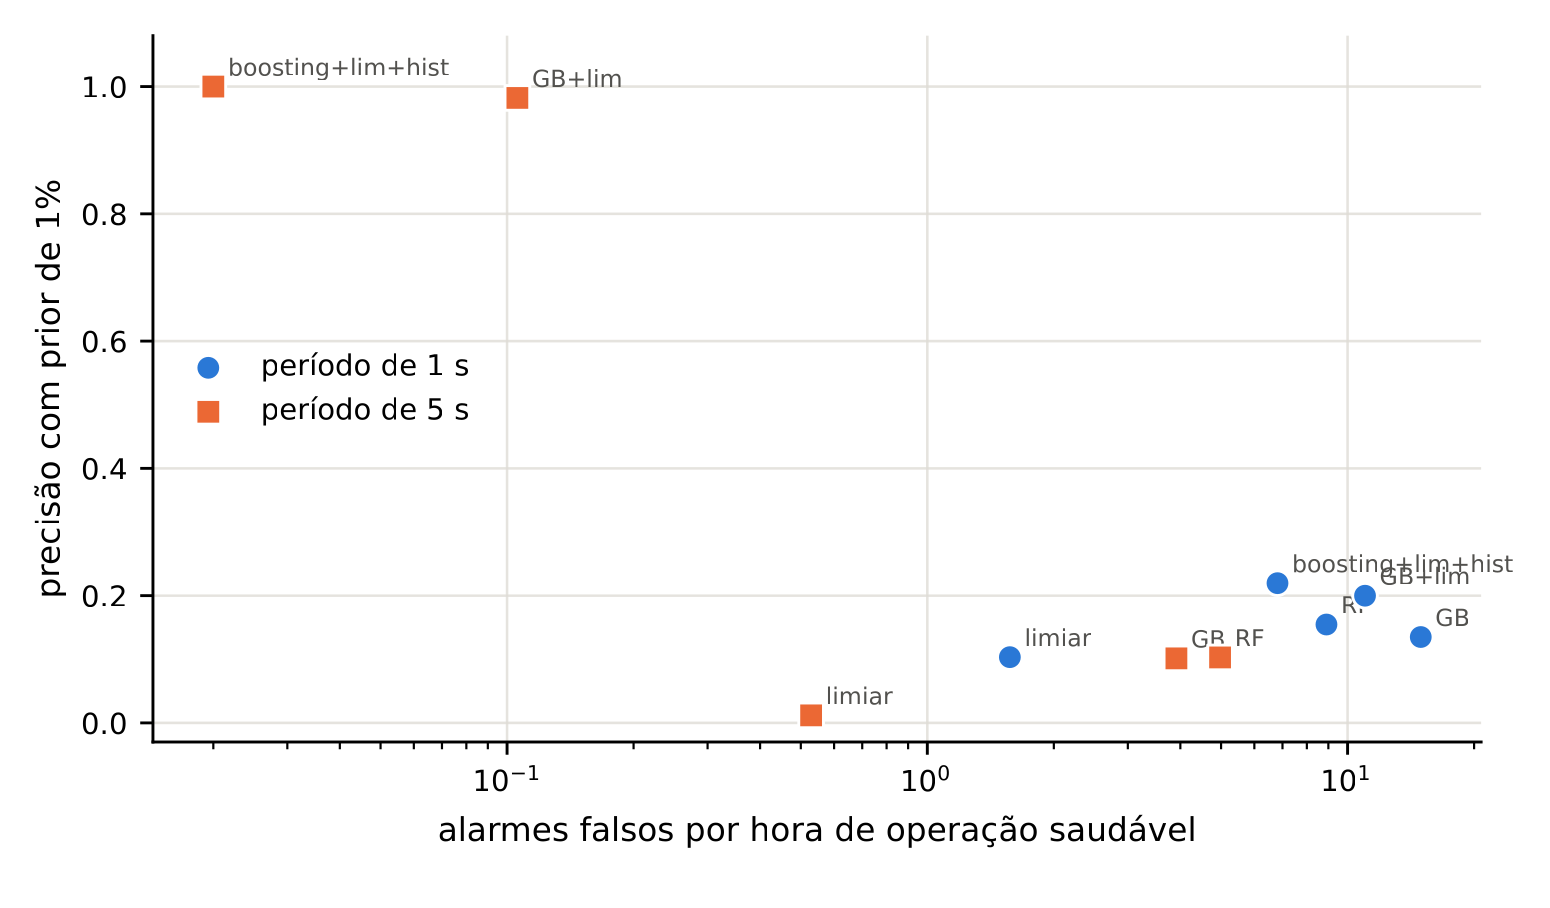
\includegraphics[width=0.8\textwidth]{figuras/qkd_precisao_alarmes.png}
\caption{Alarmes falsos por hora contra precisão sob prior de 1\%, com períodos
de decisão de 1~s e 5~s (eixo horizontal logarítmico). A mudança de regime vem
de decidir cinco vezes menos, com cinco vezes mais contagens por decisão, e não
da troca de modelo.}
\label{fig:precisao}
\end{figure}

O achado operacional central é que a precisão sob prior realista é governada
pela taxa de decisão, e não pelo modelo (Figura~\ref{fig:precisao}). Com período
de 5~s e limiar de decisão calibrado em episódios não vistos, o alarme falso vai
praticamente a zero e a precisão sob prior de 1\% passa de 0,22 para 1,00. O
preço é um atraso de dezenas de segundos e a classificação do
\textit{intercept-and-resend} fraco como deriva térmica. Calibrar o limiar sobre
os mesmos dados do ajuste produz um limiar nulo e piora o alarme falso; a
calibração em 20\% dos episódios de treino, fora do ajuste, é o que torna o
mecanismo eficaz.

\subsection{Ajuste da taxa de chave}
\label{sec:taxa}

O ajuste do transmissor é formulado como decisão sequencial. O estado tem 16
entradas: os observáveis do período anterior relativos à calibração, a
configuração corrente e duas entradas absolutas do regime de perda. As nove
ações são ajustes multiplicativos de $\mu$, $\nu$ e do \textit{clock}, e aditivos
na fração de pulsos de sinal. A recompensa é a chave que se consegue provar no
período, calculada pelos limites de isca sobre contagens binomiais finitas, e
não a taxa assintótica. O agente é um ator-crítico com vantagem generalizada
\cite{mnih2016,schulman2016}, treinado sorteando o vão entre 25 e 80~km, com
temperatura de amostragem $T=0{,}25$ escolhida em sementes de validação.

\begin{table}[ht]
\centering
\caption{Taxa de chave secreta provável (Mbit/s), média de 24 episódios de teste
por vão, com desvio-padrão entre parênteses.}
\label{tab:taxa}
\small
\begin{tabular}{lcccc}
\toprule
Vão & Comissionamento & Agente & Oráculo & Ganho \\
\midrule
25~km & 3,180 (0,451) & 3,782 (0,506) & 3,817 (0,584) & +18,9\% \\
35~km & 2,732 (0,425) & 3,092 (0,397) & 3,059 (0,417) & +13,2\% \\
50~km & 1,899 (0,319) & 2,128 (0,312) & 2,152 (0,353) & +12,1\% \\
65~km & 1,038 (0,169) & 1,138 (0,213) & 1,220 (0,244) & +9,6\% \\
80~km & 0,489 (0,072) & 0,532 (0,113) & 0,713 (0,107) & +8,8\% \\
\bottomrule
\end{tabular}
\end{table}

Até 50~km, o agente recupera mais de 90\% da distância entre a configuração de
comissionamento e o oráculo, que reotimiza a cada período com acesso ao canal
verdadeiro (Tabela~\ref{tab:taxa}); em 80~km, recupera apenas 19\%. Dois
diagnósticos produziram esse resultado. Com atributos apenas relativos à
calibração, o agente não distinguia regimes, pois uma queda de 20\% no ganho é
idêntica em 25 e em 80~km, embora os dois exijam movimentos opostos; as duas
entradas absolutas levaram o resultado em 80~km de $-14{,}7\%$ para $+1{,}6\%$, e
a escolha da temperatura de amostragem fez o resto. Um agente especialista,
treinado só em 50~km, perdia 86\% em 80~km. O comportamento aprendido é
interpretável: em vãos curtos, o agente leva a isca ao piso da faixa
($\nu\approx0{,}011$, contra 0,1 no comissionamento); em 80~km, eleva-a a
$\nu\approx0{,}25$, onde a penalidade de estatística finita passa a dominar.

\subsection{Sincronismo temporal}
\label{sec:sincronismo}

O coeficiente termo-óptico da sílica implica cerca de 40~ps de atraso por
quilômetro por kelvin; em 50~km, um kelvin desloca a chegada do pulso em 2~ns,
dez vezes a janela típica de um detector com porta. Quatro preditores foram
comparados em laço fechado com latência: nenhuma correção, recalibração
periódica, filtro alfa-beta e Ridge sobre a janela de estimativas mais o
termômetro. A pontuação é a taxa de chave que sobrevive, e não o erro do
atraso (Tabela~\ref{tab:sinc}).

\begin{table}[ht]
\centering
\caption{Taxa de chave a 50~km (Mbit/s) por sincronizador e largura de janela,
média de 12 execuções de uma hora, para detector silencioso (10~Hz de contagem
de escuro) e ruidoso ($10^6$~Hz).}
\label{tab:sinc}
\small
\begin{tabular}{llcccc}
\toprule
Escuro & Janela & Sem correção & Recalib. 60~s & Alfa-beta & Ridge + termômetro \\
\midrule
10~Hz & 200~ps & 0,136 & 1,001 & 1,464 & 1,508 \\
 & 500~ps & 0,309 & 1,631 & 1,958 & 1,971 \\
 & 1000~ps & 0,530 & 1,924 & 2,007 & 2,007 \\
$10^6$~Hz & 200~ps & 0,000 & 0,429 & 0,948 & 0,998 \\
 & 350~ps & 0,000 & 0,536 & 1,064 & 1,099 \\
 & 1000~ps & 0,000 & 0,128 & 0,253 & 0,253 \\
\bottomrule
\end{tabular}
\end{table}

Um enlace deixado sem rastreamento perde 85\% da chave em uma hora com detector
silencioso, e toda ela com detector ruidoso, efeito do coeficiente termo-óptico
e não de aprendizado de máquina. A recalibração periódica custa dos dois lados:
a janela envelhece entre varreduras, e a varredura interrompe o enlace. A margem
do preditor com termômetro é pequena e aparece onde deveria, com janela estreita
e detector ruidoso, porque só ele tem acesso à variação de temperatura.

\subsection{Validação com dados da rede de Cambridge}
\label{sec:cambridge}

Todos os resultados anteriores foram medidos no simulador do próprio trabalho.
Para confrontar a física com uma rede implantada, foram usados os dados
publicados da rede quântica de Cambridge \cite{dynes2019}\footnote{Dados sob
licença CC-BY em \url{https://doi.org/10.17863/CAM.44524}.}: 575 instantâneos
diários, de novembro de 2016 a julho de 2018, da taxa de chave e da QBER do
enlace CAPE--TREL (10,6~km, 3,9~dB; BB84 com estados-isca a 1~GHz, $\mu=0{,}4$,
$\nu=0{,}1$), e seis medidas da QBER contra a potência recebida de um canal
clássico de 100~Gbit/s na mesma fibra. Os dados não trazem observáveis por
intensidade nem ataques; o detector, portanto, não pode ser avaliado sobre eles.
O que se testa é a premissa do detector e a física compartilhada pelos
controladores (Figura~\ref{fig:cambridge}).

\begin{figure}[ht]
\centering
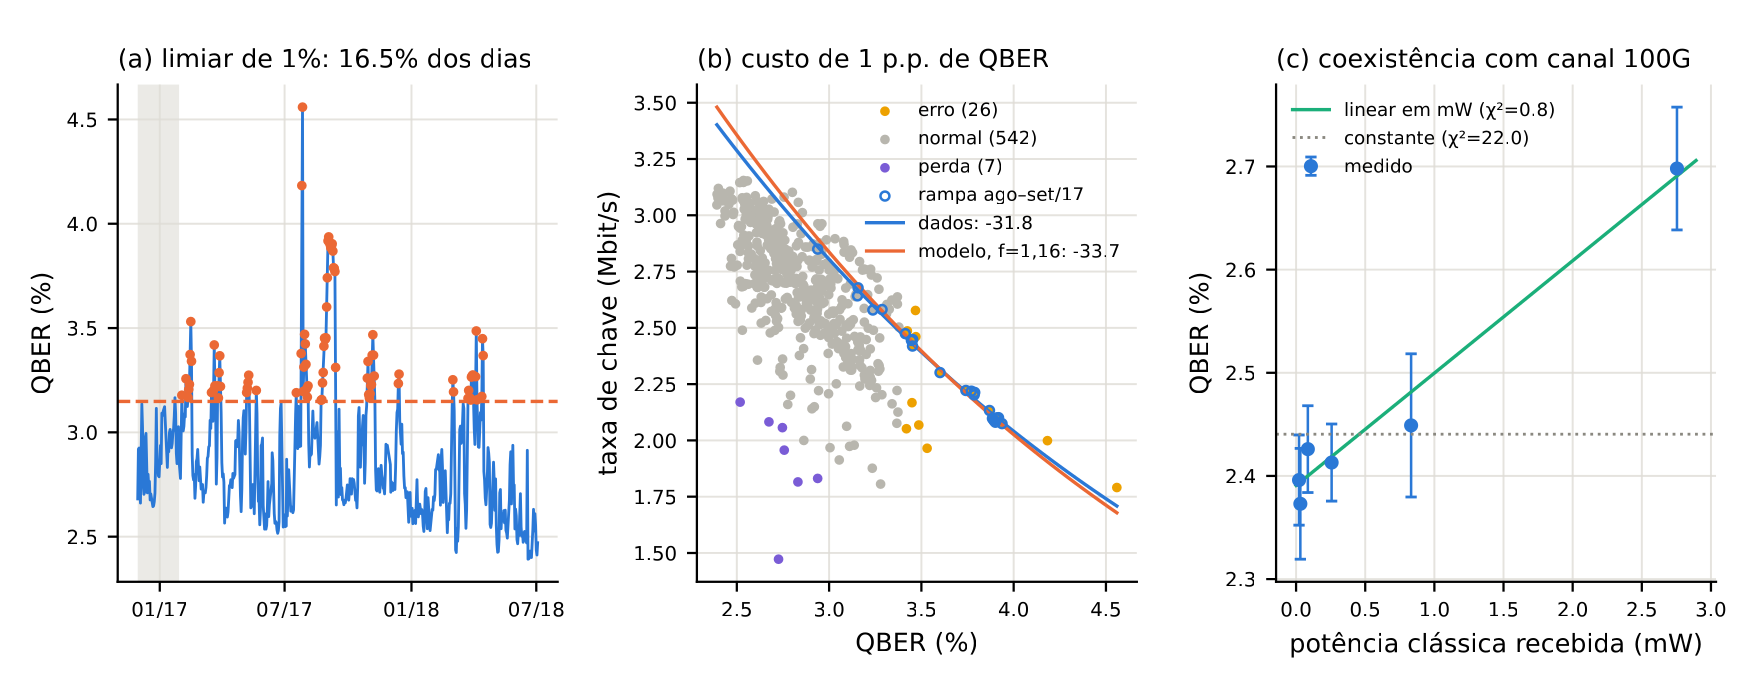
\includegraphics[width=\textwidth]{figuras/qkd_cambridge.png}
\caption{Enlace CAPE--TREL da rede de Cambridge. (a) QBER diária; em cinza, os 60 dias de comissionamento; tracejado, o limiar
calibrado para 1\% de alarme falso; pontos, os dias em que ele dispara. (b)
Taxa de chave contra QBER, com a inclinação medida na excursão de
agosto--setembro de 2017 e a prevista pelo modelo. (c) QBER contra a potência
clássica recebida, com o ajuste linear em miliwatts e a hipótese de QBER
constante. Dados de \cite{dynes2019}.}
\label{fig:cambridge}
\end{figure}

\textbf{O limiar de QBER em dias benignos.} Com 60 dias de comissionamento e
orçamento de 1\% de alarme falso, o limiar disparou em 16,5\% dos 515 dias
seguintes, em 17 episódios separados; com 90 dias de comissionamento, em 5,2\%.
Todo alarme é falso, porque todos os dias são benignos. Uma linha de base móvel
de 30 dias reduz a taxa para 2,3\%, mas aprende como normal um ataque que entre
em rampa.

\textbf{O custo de um ponto de QBER.} A taxa absoluta depende de parâmetros não
publicados, mas a sensibilidade $d\ln R/dE_\mu$ é fixada quase inteiramente
pelos termos de entropia da Eq.~\ref{eq:gllp}. Entre 22 de agosto e 12 de
setembro de 2017, a QBER subiu de 2,9\% para 3,9\% e foi corrigida em um único
dia; ao longo dessa excursão, a inclinação medida foi $-31{,}8\pm1{,}1$
($R^2=0{,}994$). O modelo prevê $-33{,}7$ com a ineficiência de reconciliação
$f=1{,}16$ usada em todo o trabalho, 6\% mais íngreme, e reproduz a medida com
$f=1{,}10$. Os dias ruins também se separam nos dois tipos de degradação do
gerador: 26 dias por erro e 7 por perda.

\textbf{Coexistência.} Sobre as seis medidas, a forma linear em miliwatts
prevista pelo espalhamento Raman ajusta os dados ($\chi^2=0{,}80$ com 4 graus
de liberdade), e a hipótese de QBER constante é rejeitada ($\chi^2=22{,}0$,
$p=0{,}0005$). A preferência depende quase só do ponto de maior potência, e a
magnitude medida é 88 vezes menor que a assumida por padrão; os limites de
potência clássica derivados com os valores padrão são, portanto, conservadores
para um receptor dessa classe.

\textbf{O limite de chave finita.} No ponto publicado (bloco peneirado de
100~Mbit, QBER de 2,4\% e $\varepsilon_{\mathrm{sec}}=10^{-10}$), a
Eq.~\ref{eq:finita} dá 0,6170 bit secreto por bit peneirado, contra 0,6472 do
limite assintótico. Com a correção de fóton único para $\mu=0{,}4$, obtêm-se
0,3495 e 0,2770 para erro de fase de fóton único igual ao observado e ao dobro
dele: o limite ideal é de 1,8 a 2,2 vezes otimista para um sistema de pulsos
coerentes. Sob o tráfego clássico máximo, a QBER de Cambridge sobe de 2,4\% para
2,7\% e a rede continua operando; o limite concorda que a excursão é barata,
com fração secreta 5,3\% menor.

% =====================================================================
\section{Arquitetura da Plataforma ORION-Q}
\label{sec:arquitetura}

\subsection{Laço de controle}

A Figura~\ref{fig:arquitetura} resume a arquitetura. As entradas (sintéticas,
\textit{replay} ou arquivo JSON medido) seguem o mesmo contrato e carregam
proveniência por observação (medida, simulada, derivada ou prevista); trocar a
fonte não concede nenhuma permissão adicional. Cada ciclo produz um
\textit{snapshot} tipado do estado da rede, com carimbo de tempo, versão e
verificação de integridade. A política ativa propõe uma ação; um supervisor de
segurança independente pode vetá-la, por exemplo forçando HALT quando a entrada
está fora do domínio de treino; e o executor aplica a decisão somente nos modos
\textit{shadow} ou simulação. Não existe modo físico: todo registro carrega o
invariante \texttt{physical\_action\_performed=false}. Todos os ciclos são
gravados em um diário SQLite com hashes.

\begin{figure}[ht]
\centering
\begin{tikzpicture}[
  font=\sffamily\scriptsize,
  box/.style={draw, rounded corners=2pt, align=center, minimum height=9mm,
              text width=24mm, fill=white},
  side/.style={box, fill=gray!10, text width=28mm},
  arr/.style={-{Stealth[length=2mm]}, thick},
  aud/.style={-{Stealth[length=2mm]}, dashed}]
  \node[box] (in) {Fontes de entrada\\sintética · \textit{replay} · JSON medido};
  \node[box, right=6mm of in] (snap) {\textit{Snapshot} tipado\\+ proveniência};
  \node[box, right=6mm of snap] (pol) {Política ativa\\(\textit{baseline} ou\\modelo aprovado)};
  \node[box, below=14mm of pol] (sup) {Supervisor de\\segurança\\(veto, OOD $\to$ HALT)};
  \node[box, left=6mm of sup] (exe) {Executor\\\textit{shadow} · simulação\\(sem modo físico)};
  \node[box, left=6mm of exe] (log) {Diário SQLite\\com hashes\\(auditoria)};
  \node[side, right=7mm of pol] (cat) {Catálogo de modelos\\OFF por padrão\\SHA-256 · sem pickle};
  \node[side, below=14mm of cat] (q05) {Fluxo de ativação\\preparar $\to$ revisar $\to$\\aprovar $\to$ ativar\\confirmação · reversão};
  \draw[arr] (in) -- (snap);
  \draw[arr] (snap) -- (pol);
  \draw[arr] (pol) -- (sup);
  \draw[arr] (sup) -- (exe);
  \draw[arr] (exe) -- (log);
  \draw[arr] (cat) -- (q05);
  \draw[arr] (q05.west) -- ++(-3.5mm,0) |- (pol.east);
  \draw[aud] (snap.south) -- ++(0,-6.5mm) -| node[pos=0.3, above, font=\sffamily\tiny]{\textit{shadow}} (log.north);
  \draw[aud] (q05.south) |- ++(0,-5mm) -| ($(log.south)+(0,0)$);
\end{tikzpicture}
\caption{Arquitetura do ORION-Q. Linhas contínuas: laço de controle;
tracejadas: registros de auditoria das sessões \textit{shadow} (recomendações
registradas, nunca aplicadas) e do fluxo de ativação.}
\label{fig:arquitetura}
\end{figure}

\subsection{Trilhas de evidência}

A plataforma separa três trilhas: telemetria óptica medida, usada somente como
observação de saúde do enlace; QBER e SKR medidos, válidos apenas dentro da
grade experimental de origem; e fidelidade de Bell simulada, restrita ao
ambiente de controle simulado. A conversão de BER, QBER ou SKR em fidelidade de
Bell é proibida, e qualquer tentativa de usar evidência óptica ou de QKD para
disparar PURIFY ou SWAP é recusada. O registro formal de reivindicações do
trabalho usa essa mesma separação: cada afirmação tem um selo (suportada,
exploratória, não suportada, refutada para os modelos avaliados ou não testada)
e aponta para evidências com hash, verificadas automaticamente.

\subsection{Admissão de modelos}

Os controladores das Seções~\ref{sec:rede} e~\ref{sec:qkd} são exportados do
qnet\_autopilot e entram na plataforma como pacotes ZIP cuja identidade é
fixada por SHA-256;
qualquer alteração exige nova revisão. O conteúdo é lido em memória, sem
extração, sem importar os \textit{scripts} fornecidos e sem desserializar
\textit{pickle}: os pesos são lidos como \textit{arrays} numéricos
(\texttt{allow\_pickle=False}), e objetos, valores não finitos e tamanhos acima
dos limites são recusados. Cada componente ganha um adaptador com contrato
explícito de domínio, cadência e horizonte, e só é admitido se reproduzir as
saídas de referência fornecidas com o modelo. O catálogo resultante tem onze
entradas, todas admitidas. O detector chegou só como \textit{pickle} e ficou
bloqueado até que se construísse uma alternativa segura: o ORION-Q o retreina com
o pipeline do próprio autor, serializa o resultado como a exportação fez e
compara os bytes com o arquivo do pacote --- idênticos ---, sem nunca
desserializá-lo; só então as 2.400 árvores são gravadas como \textit{arrays}
numéricos, lidos com \texttt{allow\_pickle=False}, e a plataforma se vincula ao
pacote conferindo o SHA-256 do membro \textit{pickle}. Todas as entradas ficam
desligadas por padrão, e a plataforma funciona sem nenhum peso externo. A Tabela~\ref{tab:admissao} resume os
contratos e a paridade verificada. A DualHead do estudo preliminar também está
disponível como pacote congelado, com leitura sem \textit{pickle} e
\textit{replay} no painel. As features de roteamento geradas no ORION-Q são
ilustrativas e não reproduzem a normalização do simulador original.

\begin{table}[ht]
\centering
\caption{Componentes admitidos no ORION-Q, contratos dos adaptadores e verificação de paridade.}
\label{tab:admissao}
\scriptsize
\begin{tabular}{>{\raggedright\arraybackslash}p{2.1cm}>{\raggedright\arraybackslash}p{2.5cm}>{\raggedright\arraybackslash}p{3.6cm}>{\raggedright\arraybackslash}p{3.5cm}}
\toprule
Componente & Modelo & Entrada $\to$ saída & Paridade conferida \\
\midrule
Sincronizador QKD & Ridge & 8 \textit{offsets} e temperaturas (passo 1~s) $\to$ \textit{offset} em +2~s & 593 previsões \\
Ator de taxa de chave & Ator 16-64-64-9 & observáveis \textit{decoy-state} $\to$ 1 de 9 ajustes limitados & features, probabilidades e ações em 40 períodos \\
Compensador de polarização & Ridge e MLP, 2 regimes (4 \textit{checkpoints}) & 48 features de rotações SO(3) (2~ms) $\to$ rotação em +40~ms & 40 mil saídas e 48 janelas \\
Roteamento e temporização & Ator-crítico, 2 \textit{checkpoints} & 11 features de estado + 23 por ação $\to$ pontuação por ação & 24 exemplos \\
Alocador híbrido & Lei de controle + persistência ou Ridge & 11 enlaces, passo 5~s, fila de 30~s $\to$ admissão por enlace & 1.440 passos e 20 \textit{snapshots} \\
Detector de ataques QKD & \textit{Boosting}, exportação segura & 17 features por período $\to$ classe e alarme & 7 sessões exportadas, byte a byte \\
\bottomrule
\end{tabular}
\end{table}

\subsection{Modos de uso de um modelo}

Um modelo admitido pode ser usado em três níveis. Na sessão \textit{offline},
o operador executa o modelo sobre uma janela explícita e compara a saída com a
persistência. No modo \textit{shadow}, as observações contínuas vêm das mesmas
plantas em que os modelos foram treinados (Seção~\ref{sec:metodologia}),
conduzidas pelo controlador vigente: a fibra com monitoramento de fótons, o
relógio com deriva térmica, o enlace \textit{decoy-state} na configuração de
comissionamento, a planta metropolitana sob admissão quântico-primeiro e a
cadeia de repetidores sob a heurística gulosa. O modelo recomenda ações, que
são registradas e avaliadas, mas nunca aplicadas. No laço fechado,
a ação do modelo altera o estado simulado. Em operação, esse nível só é
acessível pelo fluxo de ativação descrito a seguir; as campanhas de avaliação o
executam sob protocolo congelado, sem alterar o controlador ativo.

\subsection{Fluxo de ativação auditável}

Nenhuma política nova entra em vigor sem cinco etapas explícitas. (i) A
\textit{preparação} vincula a proposta à sessão de execução, à configuração
observada e ao hash da topologia, e expira em 300~s. (ii) A \textit{revisão}
confere se esse contexto ainda é válido. (iii) A \textit{aprovação} registra
uma declaração explícita do operador, com confirmação inicialmente desmarcada;
ela não autentica o operador nem autoriza atuação física. (iv) A
\textit{ativação} ocorre sob bloqueio do ciclo, dentro de uma transação SQLite:
o contexto é relido, os hashes são conferidos e a referência da política é
trocada; se a confirmação da gravação falhar ou for ambígua, a política
anterior é restaurada e novos ciclos ficam bloqueados até uma recuperação
explícita. (v) A \textit{leitura de confirmação} distingue o registro histórico
(COMMITTED) do estado vigente (ACTIVE). A \textit{reversão} prepara a política
anterior e exige nova revisão, aprovação e ativação. Um painel de auditoria
reconstrói cada decisão separando a ação pretendida, o veto do supervisor e o
resultado do executor.

O fluxo foi escrito primeiro para o limiar da política do repetidor e depois
estendido ao alvo de controle de polarização (Seção~\ref{sec:metodologia}). Ali,
a proposta de ativar um compensador aprendido só é aceita se o contrato admitir
o \textit{checkpoint} naquela planta e se o operador indicar um resumo de
campanha em laço fechado, identificado pelo hash do arquivo, no qual aqueles
mesmos pesos, identificados pelo hash dos arquivos do modelo, venceram todos os
\textit{baselines} após a correção de Holm. A revisão, a aprovação e a ativação
recalculam esses vínculos. A ativação constrói o controlador, confere que ele
reproduz a configuração aprovada e só então o coloca no laço, restaurando o
anterior se a gravação falhar. O padrão é o filtro alfa-beta, e a reversão
volta a ele pelo mesmo fluxo. Cada execução do laço fica registrada no diário
junto com a ativação sob a qual rodou.

\subsection{Implementação}

A plataforma foi escrita em Python, com PyTorch \cite{paszke2019} e Qiskit Aer
\cite{javadi2024} no núcleo científico (cerca de 23 mil linhas), uma camada de
plano de controle e console nativo em PySide6 (cerca de 39 mil linhas) e um
pacote executável para Windows. A suíte automatizada tem 3.724 testes. Em
Linux, 3.721 passam e 3 são próprios do Windows: dois valores de referência
numéricos gravados nessa plataforma e o lançador do executável. O registro de
reivindicações do estudo preliminar é verificado por 69 checagens automáticas, e o
da plataforma --- laços fechados, ponto fixo, blocagem, detector, RTL e segurança da ativação,
20 afirmações, inclusive as que não se confirmaram --- por 795 checagens sobre os
resumos das campanhas e da demonstração. As campanhas foram repetidas no Windows~11,
com os arquivos fixados originais, e comparadas número a número com as da nuvem
(Linux): as doze deram as mesmas conclusões, e onze, cada número (tolerância
relativa de $10^{-9}$, 6.698 valores); a exceção numérica é uma célula do atuador
limitado (MLP a 60~rad/s), sensível ao caminho, com QBER $1{,}6\times10^{-5}$ acima em
termos relativos. Os portões do detector e da taxa de chave exigiam igualdade de bytes
de valores simulados, que a biblioteca matemática de cada plataforma altera no último
bit; passaram a usar a tolerância declarada no protocolo, sem mudar nenhum resultado no
Linux.

% =====================================================================
\section{Avaliação na Plataforma: Metodologia}
\label{sec:metodologia}

\subsection{Níveis de evidência}

A avaliação segue três níveis cumulativos: (i) \textit{paridade}, em que o
adaptador reproduz as saídas de referência do pacote original; (ii)
\textit{shadow}, em que o modelo prevê sobre observações de uma planta que ele
não controla e é pontuado contra alvos observados depois; e (iii) \textit{laço
fechado}, em que a ação do modelo altera o estado simulado e o efeito é medido
na variável controlada. Um nível superior não é inferido de um inferior:
paridade não indica ganho, e erro de previsão menor não indica melhor controle.

\subsection{Protocolo das campanhas shadow}

Cada campanha teve protocolo gravado com hash antes da primeira inferência,
sementes fixas (100 a 109) e nenhum treino, ajuste ou seleção sobre os
resultados. O sincronizador foi avaliado em seis cenários artificiais com 128
quadros por execução, contra persistência e média dos oito \textit{offsets}
anteriores. O compensador foi avaliado em seis cenários, quatro
\textit{checkpoints} e dez sementes (240 execuções), com erro medido pelo
ângulo geodésico em SO(3), contra persistência e contra velocidade angular
constante estimada dos 15 incrementos anteriores. Um cenário só foi considerado
favorável quando o modelo reduziu o erro médio em pelo menos 5\% contra cada
\textit{baseline}, venceu em pelo menos 8 de 10 sementes e manteve cobertura de
pelo menos 90\% em todas as sementes. Esses são critérios descritivos de
engenharia, não testes de significância.

\subsection{Protocolo em laço fechado}

\textbf{As plantas dos modelos.} As duas versões do qnet\_autopilot que
produziram os pesos --- a de rede (roteamento, compensador e alocador) e a de
QKD (ator de taxa de chave, sincronizador e detector) --- foram incorporadas ao
repositório do ORION-Q como pacotes independentes, copiados byte a byte a partir
dos arquivos do autor, com um manifesto que registra o hash de cada arquivo;
só as poucas importações absolutas foram renomeadas, para que as duas versões
convivam no mesmo processo. As suítes do autor passam sobre as cópias (878 e 926
testes, com o SeQUeNCe onde é exigido). Os registros de resultado do autor
(tabelas e \textit{logs}, sem \textit{pickles}) também foram incorporados, como
referência dos portões descritos a seguir. Com isso, cada laço fechado do
ORION-Q roda sobre a planta em que o modelo foi treinado, e não sobre um
produtor escrito para a plataforma. A planta da polarização é uma transcrição do
modelo de fibra (tom com harmônicos, deriva térmica de Ornstein-Uhlenbeck,
saltos, monitoramento com 400 fótons por base reprojetado em SO(3)); a mesma
semente produz a mesma trajetória que o pacote do autor, bit a bit. As demais
plantas são o próprio código do autor.

\textbf{Regras comuns.} Todo laço segue as mesmas cinco regras.
(i) Um contrato admite o modelo só na planta que seus metadados declaram e
recusa qualquer diferença (fibra, período, horizonte, fótons; caixa de ações e
tempo morto; vão de treino; plano de enlaces; topologia e custos).
(ii) O ORION-Q entrega ao modelo apenas o que um controlador real veria (a
estimativa de rotação, os observáveis publicados do período anterior, a
estimativa do atraso, a telemetria da planta metropolitana, as características
do estado e das ações legais), nunca o estado oculto da planta.
(iii) Um supervisor fica entre o modelo e a planta; quando o modelo é recusado,
um controlador de reserva assume (filtro alfa-beta, manutenção dos parâmetros,
quântico-primeiro, heurística gulosa).
(iv) Antes de qualquer pontuação, a campanha regenera pela réplica do ORION-Q
resultados que o autor publicou ou exportou --- episódios inteiros, tabelas do
manuscrito ou valores declarados nos metadados --- e para se algum não for
reproduzido.
(v) O protocolo é congelado em arquivo com hash; as sementes de avaliação são
novas, disjuntas das de treino, validação e teste do autor; as comparações usam
o teste de permutação de sinais pareado e exato, com correção de Holm, e
intervalos por \textit{bootstrap} sobre sementes.

\textbf{Compensador de polarização.} O compensador ganhou no ORION-Q um alvo de
controle próprio, separado da política do repetidor. A cada 2~ms, o controlador
recebe a estimativa de rotação e as covariáveis e propõe a rotação da fibra
40~ms à frente. O supervisor recusa propostas não finitas ou fora de SO(3) e
mantém o comando anterior; limita a variação geodésica entre comandos
consecutivos a $\pi/2$ por período, acima da maior variação da própria fibra
numa trajetória de referência (1,24~rad); e, após oito recusas seguidas, degrada
até o fim da execução para o filtro alfa-beta, que roda em espera quente.
Reativar o modelo exige nova ativação. O protocolo principal\footnote{Arquivo
\texttt{configs/optional\_models/polarisation\_closed\_loop\_v1.json}, SHA-256
\texttt{0b7b12b5\ldots{}79d9f4}; o do ponto de desenvolvimento difere só no ponto,
nos \textit{checkpoints} e nas sementes de reprodução.} usa 20 sementes de planta
novas (1000 a 1019) e execuções de 20~s, com atuador ideal. Os comparadores são
os da Seção~\ref{sec:compensador}: sem compensação, persistência e filtro
alfa-beta, este ressintonizado por busca em grade ($11\times8$ pares) em quatro
sementes de ajuste separadas, numa grade estendida para baixo em relação à do
qnet\_autopilot, porque ali o ótimo caía na borda. O desfecho primário é a QBER
média por semente (Eq.~\ref{eq:erro_pol}); os secundários são o ângulo residual,
a disponibilidade (fração do tempo com QBER abaixo de 11\%) e a taxa de chave.
O teste é unilateral, com Holm sobre as seis comparações. O portão exige que
cada \textit{checkpoint} reproduza, até $10^{-9}$, a QBER retida declarada em
seus metadados. Uma sétima execução por semente injeta 50 passos de saída
inválida no Ridge a partir de $t=5$~s. A mesma campanha foi repetida no ponto de
desenvolvimento. Uma terceira campanha coloca entre o supervisor e a fibra o
atuador limitado do autor --- três retardadores X-Y-X com velocidade e curso
finitos e \textit{reset} sem fim --- e varre a velocidade de 30 a
10.000~rad/s nos dois pontos, com o alfa-beta ressintonizado para cada
dispositivo e teste bilateral; seu portão é a varredura de velocidade do
próprio autor.

\textbf{Ator de taxa de chave e sincronizador.} O ator roda no ambiente
\textit{decoy-state} do autor no ponto de referência (50~km nominais, 1~dB de
perda extra, tempo morto de 50~ns, 240 períodos de 1~s por episódio), nos vãos
de 25, 35, 50, 65 e 80~km. A cada período, o ORION-Q pede à réplica um dos nove
ajustes limitados e confere, bit a bit, que os parâmetros adotados pela planta
são os propostos. O sincronizador roda no laço de porta do autor a 50~km, com
2.000 fótons por estimativa e 2~s de latência; as sete primeiras atualizações
usam a regra de aquecimento do próprio autor, registrada. Os portões regeneram
o episódio exportado de 40 períodos e as Tabelas~\ref{tab:taxa}
e~\ref{tab:sinc}. As sementes novas são 950000--950019 (taxa de chave) e
600--619 (sincronismo); as hipóteses são unilaterais, ator contra comissionamento
por vão e Ridge contra alfa-beta por janela e contagem de escuro.

\textbf{Alocador e roteamento.} O alocador roda na planta metropolitana do autor
com a contabilidade de chave finita declarada pela exportação, contra
quântico-primeiro, admissão estática, limiar reativo ressintonizado e
clássico-primeiro. Seus portões regeneram os quatro episódios exportados e o
ponto da fronteira retraçada com chave finita. O agente de roteamento roda no
ambiente analítico de repetidores do autor, nas duas variantes exportadas
(prazo nominal e prazo quádruplo); os portões regeneram as 2.091 decisões dos
episódios exportados e as duas tabelas retidas. Como o manuscrito descreve
empate com a melhor heurística, o teste do roteamento é bilateral, sobre 20
blocos de 50 episódios. Uma segunda campanha põe o próprio SeQUeNCe no lugar do
ambiente analítico, pelo executor de eventos discretos do autor: cada primitiva
escolhida pela réplica é resolvida pelos protocolos do SeQUeNCe. Seus portões
regeneram as 480 linhas da comparação do autor entre os dois simuladores e a
medida do custo de uma tentativa de \textit{heralding}, com os pesos do agente da
fase 2 do arquivo do autor, e exigem que o lado analítico das mesmas 1.000
requisições reproduza a primeira campanha.

\textbf{Detector.} O detector é um monitor e não fecha laço: o que se avalia é
se a réplica é o detector do autor e como ele se sai em sessões que ninguém usou.
O portão regenera o conjunto de sessões do autor e reproduz as métricas por
classe da Tabela~\ref{tab:detector}, as tabelas do divisor de feixe, dos casos
difíceis e da confusão e as duas calibrações, com as funções de pontuação do
próprio autor sobre a réplica. A avaliação usa dois conjuntos novos de 168
episódios. O gerador dá ao episódio $i$ do conjunto de semente $s$ o fluxo
aleatório $s+i$; como o autor usou os fluxos 0 a 167, conjuntos de semente 1 ou 2
repetiriam os episódios de treino deslocados de um, e a avaliação usa as
sementes 1000 e 2000. O limiar de QBER mantém a calibração do autor. A hipótese
primária compara, por episódio com evento, a fração dos períodos marcados como
ataque pelo detector implantado e pelo limiar (teste do sinal exato, Holm sobre
os dois conjuntos). A taxa de variação da temperatura do autor é uma diferença
central: a variável do período $t$ usa a temperatura de $t+1$, o que um monitor em
tempo real não tem. Uma segunda campanha recalcula, para cada período, as
variáveis com a própria função do autor sobre o registro até ele e compara as duas
versões nos mesmos conjuntos e com o mesmo modelo, sem retreinar; o portão exige
que as 15 variáveis sem antecipação sejam idênticas bit a bit.

\textbf{Ponto fixo.} O porte do compensador para ponto fixo
(Seção~\ref{sec:compensador}) foi medido pelo autor só no ponto de desenvolvimento.
No ORION-Q, os compensadores são reconstruídos a partir dos \textit{arrays} do
pacote e passam pela quantização do próprio autor; o portão regenera a varredura
de largura de palavra do autor, linha a linha. Os formatos são calibrados nas
sementes de ajuste, e cada configuração roda nas 20 sementes de avaliação, com a
predição projetada na rotação mais próxima antes do supervisor, que recusa o que
está fora de SO(3). A hipótese primária é a não inferioridade, com margem de 5\%,
do ponto fixo de 16 bits com CORDIC de 8 estágios --- a configuração do RTL ---
em relação ao ponto flutuante (Holm sobre quatro casos).

\textbf{Blocagem.} O controlador de blocagem (Seção~\ref{sec:blocagem}), na versão
que pode pular segmentos, liquida a QBER por amostra do laço supervisionado do
ORION-Q, nas mesmas 20 sementes e com os mesmos compensadores, contra
temporizadores de 0,1 a 20~s e os dois oráculos do autor. Os portões regeneram,
pelo laço do ORION-Q, a tabela de blocagem do autor nas suas 12 sementes e, pelo
laço do autor, a de estresse sob vibração crescente. O melhor temporizador é
escolhido com retrospectiva, a favor dele. Com persistência, a hipótese é de
superioridade sobre o melhor temporizador; com os compensadores aprendidos, de não
inferioridade com margem de 1\% (unilaterais, Holm por família).

\textbf{Verilog.} O pacote de rede traz o RTL do compensador (multiplicador-acumulador
e CORDIC) com um \textit{testbench} que nunca havia sido executado; o de QKD traz
o preditor do sincronizador e o classificador em árvores podado do detector. Cada
bloco foi simulado no Icarus Verilog contra a referência em ponto fixo do próprio
autor e sintetizado no Yosys para a família Xilinx~7 (mapeamento lógico, sem
posicionamento nem análise de tempo).

% =====================================================================
\section{Avaliação na Plataforma: Resultados}
\label{sec:resultados}

\subsection{Paridade}

As onze configurações admitidas reproduziram as saídas de referência de seus
pacotes nos volumes indicados na Tabela~\ref{tab:admissao}; no detector, as sete
sessões de exemplo exportadas saíram idênticas byte a byte, entrada, gabarito e
saída. A paridade confirma que a plataforma executa os modelos
como foram entregues; ela não é evidência de desempenho.

\subsection{Campanhas shadow}

\begin{figure}[ht]
\centering
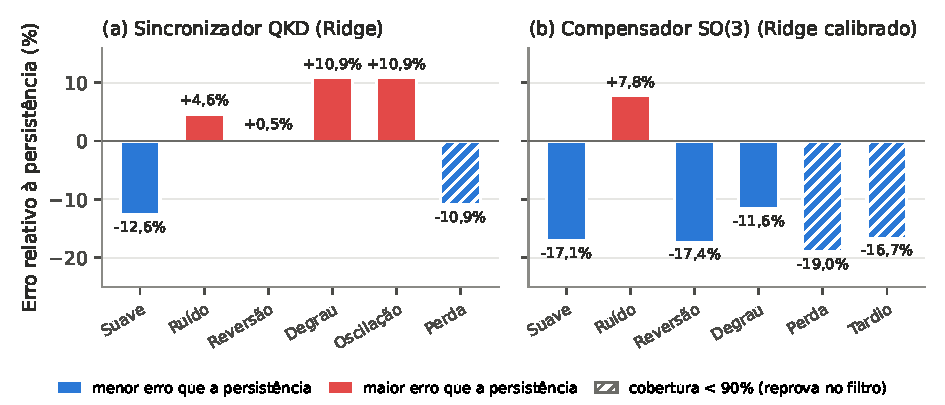
\includegraphics[width=\textwidth]{figuras/shadow_campanhas.pdf}
\caption{Erro de previsão relativo à persistência por cenário (negativo:
modelo melhor). (a) Sincronizador, MAE do \textit{offset} a +2~s; (b)
compensador Ridge do regime calibrado, erro angular a +40~ms. Barras
hachuradas reprovaram no critério de cobertura.}
\label{fig:shadow}
\end{figure}

A Figura~\ref{fig:shadow} resume as duas campanhas, feitas com os produtores
artificiais que o console usava até então; eles foram depois substituídos pelas
plantas do autor (Seção~\ref{sec:discussao}). O sincronizador atendeu ao
critério apenas no cenário suave, com MAE 12,6\% menor que a persistência.
Com ruído independente, degrau e oscilação rápida, foi 4,6\%, 10,9\% e 10,9\%
pior; na reversão de deriva, empatou em média (5 vitórias em 10). Com perda de
pacotes, o erro nos pares disponíveis foi 10,9\% menor, mas a cobertura caiu
para 80,7\%.

O compensador Ridge atendeu ao critério em 6 dos 24 grupos: nos dois regimes,
nos cenários suave, reversão térmica e degrau, com reduções de erro entre
11,6\% e 17,4\% frente à persistência no regime calibrado e vitória em todas as
sementes. Com ruído na rotação, o Ridge calibrado foi 7,8\% pior que a
persistência. Com perda de pacotes ou resultados tardios, venceu nos pares
disponíveis, mas a cobertura de 73,3\% reprovou todos os
\textit{checkpoints}. O MLP perdeu para os dois \textit{baselines} em todas as
sementes e cenários (0 de 120 vitórias contra cada um) nesta família
artificial, embora empate com o Ridge no simulador de origem
(Seção~\ref{sec:compensador}); a diferença é discutida na
Seção~\ref{sec:discussao}.

\subsection{Compensador em laço fechado}

O contrato admitiu os dois \textit{checkpoints} calibrados e recusou os dois de
desenvolvimento nessa planta. No portão de reprodução, o laço supervisionado
repetiu a QBER retida declarada pelo Ridge (0,0132653151857) e pelo MLP
(0,0136375117637) com diferença da ordem de $10^{-16}$. A ressintonia escolheu
$\alpha=0{,}01$ e $\beta=0$, o que torna o filtro uma persistência suavizada. Com
40~ms de atraso, 2,4 períodos do tom de 60~Hz, estimar velocidade não ajuda. Nas
sementes da Tabela~\ref{tab:comp_cal}, esse filtro chega a 0,0441, contra
0,0461 do filtro ressintonizado na grade original: o \textit{baseline} desta
campanha é mais forte que o do manuscrito.

\begin{table}[ht]
\centering
\caption{Compensação em laço fechado supervisionado no ORION-Q, ponto calibrado:
20 sementes novas de 20~s. IC de 95\% por \textit{bootstrap} sobre sementes.
Disp.\ é a fração do tempo com QBER abaixo de 11\%; a chave é a taxa
assintótica do BB84 com taxa peneirada de 100~kbit/s; o resíduo é o ângulo
médio da rotação residual.}
\label{tab:comp_lf}
\small
\begin{tabular}{lcccc}
\toprule
Controlador & QBER média [IC 95\%] & Disp. & Chave (kbit/s) & Resíduo (mrad) \\
\midrule
Ridge & \textbf{0,0131} [0,0128; 0,0134] & 99,9\% & \textbf{80,1} & 253 \\
MLP & 0,0134 [0,0131; 0,0138] & 99,9\% & 79,7 & 257 \\
Alfa-beta (ressint.) & 0,0436 [0,0429; 0,0442] & 94,4\% & 50,1 & 481 \\
Sem compensação & 0,0836 [0,066; 0,106] & 75,1\% & 34,9 & 659 \\
Persistência & 0,1217 [0,119; 0,124] & 54,5\% & 19,4 & 835 \\
\bottomrule
\end{tabular}
\end{table}

A Tabela~\ref{tab:comp_lf} mostra o resultado. Os dois modelos venceram os três
\textit{baselines} em todas as 20 sementes. Contra o alfa-beta, a QBER do Ridge
ficou 3,33 vezes menor (IC 95\% 3,24--3,42) e a do MLP, 3,24 vezes menor
(3,16--3,33); contra a ausência de compensação, 6,4 e 6,2 vezes; contra a
persistência, 9,3 e 9,1 vezes. Nas seis comparações o $p$ exato foi $2^{-20}$
(o menor possível com 20 sementes) e o $p$ de Holm, $5{,}7\times10^{-6}$. A
razão contra o alfa-beta fica próxima da registrada no qnet\_autopilot (3,47,
Tabela~\ref{tab:comp_cal}), agora com sementes novas, um \textit{baseline} mais
forte e o supervisor no caminho. A taxa de chave do Ridge foi 1,6 vez a do
alfa-beta. Na planta certa, o MLP empatou com o Ridge (2,6\% acima), como no
ambiente de origem, e não perdeu em todas as sementes como nas campanhas
\textit{shadow}.

O supervisor quase não atuou nas execuções normais: de um milhão de comandos,
nenhum foi recusado e dois foram limitados em taxa, ambos num salto grande da
fibra. Na falha injetada, ele recusou as oito primeiras saídas inválidas mantendo
o último comando e degradou para o alfa-beta em $t=5{,}014$~s nas 20 execuções.
Nenhuma proposta inválida chegou à planta, e a QBER média dessas execuções
(0,0360) ficou entre a do Ridge e a do filtro, que assumiu os 15~s restantes.

\subsection{Segundo ponto de operação e atuador limitado}

Repetida no ponto de desenvolvimento, com os \textit{checkpoints} daquele ponto,
a campanha deu o mesmo quadro: o contrato admitiu os dois \textit{checkpoints} de
desenvolvimento e recusou os calibrados; a reprodução da QBER retida declarada
ficou abaixo de $10^{-16}$; e o Ridge (0,0076) e o MLP (0,0072) ficaram 4,75 e
5,00 vezes abaixo do alfa-beta ressintonizado (0,0361; IC 95\% 4,53--4,96 e
4,78--5,24), em 20 de 20 sementes, dentro da faixa do manuscrito (5,2; IC
4,7--5,8, Tabela~\ref{tab:comp_dev}).

\begin{table}[ht]
\centering
\caption{Compensação com o atuador limitado do autor: razão entre a QBER do
alfa-beta ressintonizado para cada dispositivo e a do Ridge, 20 sementes novas.
Acima de 1, o modelo é melhor. Negrito: diferença significativa após Holm
(bilateral).}
\label{tab:atuador}
\small
\begin{tabular}{lcccccccc}
\toprule
rad/s & 30 & 60 & 120 & 250 & 500 & 1.000 & 3.000 & ideal \\
\midrule
Desenvolvimento & \textbf{0,77} & \textbf{0,78} & \textbf{1,18} & \textbf{1,83} & \textbf{2,57} & \textbf{3,35} & \textbf{4,75} & \textbf{4,75} \\
Calibrado & \textbf{0,91} & \textbf{0,91} & 0,97 & \textbf{1,21} & \textbf{1,64} & \textbf{2,26} & \textbf{3,33} & \textbf{3,33} \\
\bottomrule
\end{tabular}
\end{table}

Com o atuador do autor entre o supervisor e a fibra
(Tabela~\ref{tab:atuador}), o resultado passa a depender do dispositivo. Até
60~rad/s, o filtro clássico vence em todas as sementes nos dois pontos: o
dispositivo lento filtra o comando como um passa-baixas, e o preditor, que pede
o movimento necessário para seguir a vibração (cerca de 15.600~rad em 20~s no
ponto calibrado, contra 640 do filtro), recebe uma correção atrasada e parcial.
O modelo passa a vencer a partir de 120~rad/s no ponto de desenvolvimento e de
250~rad/s no calibrado, que empata a 120~rad/s; a partir de cerca de
3.000~rad/s, o resultado é o do atuador ideal. O ponto calibrado exige um
dispositivo mais rápido porque seus harmônicos de 120 e 180~Hz pedem taxas
maiores. O manuscrito, com o filtro fixo e quatro sementes, situava o
cruzamento entre 120 e 250~rad/s no ponto de desenvolvimento; com 20 sementes e o
filtro ressintonizado por dispositivo, a vantagem já é significativa a
120~rad/s ali, e o ponto calibrado, antes não medido, cruza entre 120 e
250~rad/s. Os \textit{resets} disparam com frequência sob o preditor, mas ocupam
no máximo 3\% do tempo e não mudam a ordenação.

\subsection{Reprodução dos resultados publicados}

Antes de qualquer pontuação em sementes novas, cada campanha regenerou pela
réplica do ORION-Q, na planta do autor, resultados que o próprio autor publicou
ou exportou (Tabela~\ref{tab:portoes}). Nenhum portão falhou. Dois detalhes
tornaram a reprodução possível e não estavam documentados como tal: o exemplo
exportado do ator de taxa de chave amostra com um gerador separado, semeado com
a semente do episódio, e as tabelas de avaliação do autor usam o gerador de uma
política recém-construída; conhecidas essas convenções, as ações sorteadas
também se reproduzem, o que a paridade \textit{offline} não conferia. No
sincronismo, o \textit{script} do autor reajusta o Ridge com ruído de medida sem
semente, de modo que os coeficientes exportados diferem dos da tabela em até
0,013; mesmo assim, as 24 entradas se reproduzem na precisão publicada.

\begin{table}[ht]
\centering
\caption{Portões de reprodução: resultados do autor regenerados pelo ORION-Q
na planta de origem antes de cada campanha.}
\label{tab:portoes}
\small
\begin{tabular}{p{3.2cm}p{7.6cm}p{2.6cm}}
\toprule
Componente & Resultado regenerado & Divergência \\
\midrule
Compensador & QBER retida declarada nos metadados, 2 pontos (6 e 8 sementes) & $\leq 6\times10^{-17}$ \\
Compensador + atuador & varredura de velocidade do autor: 4 compensadores $\times$ 9 dispositivos & $\leq 3\times10^{-17}$ \\
Ator de taxa de chave & episódio exportado de 40 períodos (ações sorteadas, parâmetros, bits de chave) & 0 \\
 & Tabela~\ref{tab:taxa}: 15 médias e desvios & na precisão publicada \\
Sincronizador & Tabela~\ref{tab:sinc}: 24 entradas, 4 sincronizadores & na precisão publicada \\
Alocador & 4 episódios exportados e o ponto de cobertura 1 da fronteira com chave finita & 0 \\
Roteamento & 2.091 decisões dos 48 episódios exportados; 2 tabelas retidas & 0 e $6\times10^{-17}$ \\
Compensador em ponto fixo & varredura de largura de palavra do autor: 20 linhas $\times$ 10 colunas & $3\times10^{-16}$ (relativa) \\
Detector & 7 sessões exportadas; métricas por classe de 4 detectores da Tabela~\ref{tab:detector} (240 valores), divisor de feixe, casos difíceis, confusão e calibrações & 0 \\
\bottomrule
\end{tabular}
\end{table}

\subsection{Taxa de chave e sincronismo em laço fechado}

\begin{table}[ht]
\centering
\caption{Ator de taxa de chave em laço fechado no ORION-Q: 20 episódios novos de
240~s por vão (Mbit/s). O oráculo lê o canal verdadeiro e é só referência.}
\label{tab:taxa_lf}
\small
\begin{tabular}{lccccc}
\toprule
Vão & Estático & Ator & Oráculo & Ator/estático [IC 95\%] & $p$ de Holm \\
\midrule
25~km & 3,245 & \textbf{3,761} & 3,895 & 1,159 [1,092; 1,222] & $3{,}9\times10^{-4}$ \\
35~km & 2,670 & \textbf{3,033} & 3,116 & 1,136 [1,081; 1,197] & $1{,}3\times10^{-4}$ \\
50~km & 1,855 & \textbf{2,134} & 2,208 & 1,150 [1,096; 1,215] & $8{,}6\times10^{-5}$ \\
65~km & 0,989 & \textbf{1,195} & 1,265 & 1,208 [1,121; 1,302] & $3{,}9\times10^{-4}$ \\
80~km & 0,488 & 0,528 & 0,681 & 1,082 [0,959; 1,201] & 0,10 \\
\bottomrule
\end{tabular}
\end{table}

Em sementes novas, o ator supera a configuração de comissionamento de 25 a
65~km, com ganho de 13,6\% a 20,8\% e vitória em 17 ou 18 de 20 episódios,
fechando de 75\% a 81\% da distância até o oráculo (Tabela~\ref{tab:taxa_lf}).
A 80~km a vantagem média (8,2\%) não se distingue de zero, e a lacuna fechada
cai para 21\%, o que concorda com os 19\% da Tabela~\ref{tab:taxa}. O
comportamento aprendido é o descrito na Seção~\ref{sec:taxa}: nos vãos curtos a
isca termina no piso ($\nu\approx0{,}011$) e a fração de pulsos de sinal sobe;
a 80~km a isca sobe a $\nu\approx0{,}27$. Em 24.000 períodos, todas as
propostas foram conferidas contra a planta e o contrato não recusou nenhuma; com
recusas injetadas, o supervisor desligou o ator no oitavo período recusado e o
transmissor manteve os últimos parâmetros conferidos.

No sincronismo, em 20 execuções novas de uma hora a 50~km, o Ridge superou o
filtro alfa-beta em todas as execuções das oito configurações (quatro larguras
de janela, detector silencioso e ruidoso; $p$ de Holm $7{,}6\times10^{-6}$).
A margem, porém, só é relevante onde a Seção~\ref{sec:sincronismo} previu: com
janela de 200~ps e detector ruidoso, 5,1\% (0,999 contra 0,950~Mbit/s); com
janela de 1~ns, menos de 0,03\%. O efeito grande continua sendo o do
rastreamento em si: sem correção, a chave fica 72\% a 90\% abaixo com detector
silencioso e vai a zero com detector ruidoso.

\subsection{Alocação e roteamento em laço fechado}

\begin{table}[ht]
\centering
\caption{Alocador em laço fechado na planta metropolitana com chave finita: 20
episódios novos de 30~min. Frações servidas da demanda de chave e de tráfego
clássico. Convenção A: demanda da semente 0 (tabelas do autor); B: demanda da
semente do episódio (episódios exportados).}
\label{tab:aloc_lf}
\small
\begin{tabular}{lcccc}
\toprule
 & \multicolumn{2}{c}{Convenção A} & \multicolumn{2}{c}{Convenção B} \\
Política & Chave & Clássico & Chave & Clássico \\
\midrule
Alocador (persistência) & 0,458 & \textbf{0,233} & 0,496 & \textbf{0,249} \\
Alocador (Ridge) & 0,458 & 0,234 & 0,496 & 0,247 \\
Quântico-primeiro & 0,463 & 0,096 & 0,501 & 0,095 \\
Limiar reativo (0,02--0,04) & 0,362 & 0,588 & 0,393 & 0,587 \\
Admissão estática 0 & 0,468 & 0 & 0,503 & 0 \\
Admissão estática 0,25 & 0,345 & 0,512 & 0,376 & 0,518 \\
Clássico-primeiro & 0,096 & 1,000 & 0,112 & 1,000 \\
\bottomrule
\end{tabular}
\end{table}

O alocador revisado repetiu no laço fechado o resultado principal do manuscrito
(Tabela~\ref{tab:aloc_lf}). Contra a política que silencia o canal clássico
sempre que há chave devida, ele carregou 2,4 vezes (A) e 2,6 vezes (B) o tráfego
clássico, servindo chave dentro de 0,5 ponto percentual; as duas hipóteses
primárias (tráfego clássico maior; chave não inferior com margem de 2 pontos)
valeram nas 20 sementes, para as duas configurações e as duas convenções ($p$ de
Holm $7{,}6\times10^{-6}$). Para servir a mesma chave, a admissão estática teria
de ficar próxima de zero e carregaria 5,6 vezes menos tráfego clássico (A; IC
95\% 5,1--6,2). Esse número não substitui os 2,7 vezes da
Seção~\ref{sec:alocador}, que são uma média sobre a sobreposição das fronteiras
ao longo da cobertura, e apenas a cobertura 1 é um modelo revisado. A previsão
Ridge ficou a menos de 0,2 ponto da persistência em chave e em tráfego, como o
autor registrou: o ganho é da lei de controle.


\begin{table}[ht]
\centering
\caption{Agente de roteamento em laço fechado: 1.000 episódios novos por
variante, no gêmeo analítico e no SeQUeNCe (mesmas requisições). Taxa de sucesso
e retorno bruto médio; comparação primária contra a heurística gulosa por teste
bilateral sobre 20 blocos de 50 episódios.}
\label{tab:rot_lf}
\small
\begin{tabular}{llcccc}
\toprule
Variante & Política & Sucesso & Retorno & $p$ de Holm vs.\ gulosa & Sucesso no \\
 & & & bruto & (sucesso; retorno) & SeQUeNCe \\
\midrule
Nominal & agente ($T=1$) & 20,4\% & $-0{,}416$ & 0,010; 0,016 & 19,0\% \\
 & gulosa de fidelidade & \textbf{23,4\%} & $\mathbf{-0{,}382}$ & -- & \textbf{22,9\%} \\
 & caminho mais curto & 23,4\% & $-0{,}382$ & -- & 22,9\% \\
 & limiar 0,90 & 7,2\% & $-0{,}635$ & -- & 7,4\% \\
Prazo $\times4$ & agente (guloso) & \textbf{45,1\%} & $\mathbf{-0{,}023}$ & 1,0; 1,0 & 45,4\% \\
 & gulosa de fidelidade & 45,0\% & $-0{,}025$ & -- & \textbf{46,7\%} \\
 & caminho mais curto & 29,9\% & $-0{,}229$ & -- & 29,6\% \\
 & limiar 0,90 & 22,6\% & $-0{,}434$ & -- & 22,5\% \\
\bottomrule
\end{tabular}
\end{table}

No roteamento, a campanha refinou o resultado do manuscrito
(Tabela~\ref{tab:rot_lf}). Com prazo quádruplo e custo por tentativa invariante,
o agente guloso empata com a heurística gulosa de fidelidade e supera as demais
(45,1\% contra 29,9\% do caminho mais curto, em 19 de 20 blocos). No prazo
nominal, porém, o agente amostrado com $T=1$ fica 3 pontos abaixo da heurística
(20,4\% contra 23,4\%, 3 blocos a favor e 15 contra; $p$ de Holm 0,010). A
tabela retida do próprio pacote já mostrava essa diferença (21,75\% contra
24\%), lida como empate com 400 episódios; com 1.000 episódios e teste pareado,
ela é real. A conclusão sobre o roteamento não muda --- o aprendizado não supera
a melhor regra simples ---, mas o empate vale apenas no prazo longo.

Com o SeQUeNCe como planta, os portões regeneraram as 480 linhas da comparação do
autor com erro zero --- o SeQUeNCe usado é o dele --- e o lado analítico repetiu a
primeira campanha exatamente. O gêmeo, cobrando as 4,1 travessias por tentativa que
o autor mediu, prevê o SeQUeNCe: nenhuma das oito taxas de sucesso da
Tabela~\ref{tab:rot_lf} muda de forma significativa entre os dois simuladores
(de $-1{,}4$ a $+1{,}7$ ponto; $p$ de Holm 1,0), e os dois ofereceram as mesmas
ações legais em todos os passos de 8.000 episódios. O que o SeQUeNCe acrescenta é
resolução: o agente fica abaixo da heurística nos dois prazos, 19,0\% contra
22,9\% no nominal ($p$ de Holm $1\times10^{-4}$) e 45,4\% contra 46,7\% no prazo
quádruplo ($p$ de Holm 0,004). Neste, as duas políticas seguem a mesma trajetória
em 892 das 1.000 requisições; nas que diferem, a heurística entrega em 13 e o
agente em nenhuma. O empate do prazo longo é, portanto, um resultado do gêmeo.

\subsection{Detector em sessões novas}

\begin{table}[ht]
\centering
\caption{Detector em dois conjuntos novos de sessões (144 episódios pontuados
cada), com a réplica segura. Detecção: fração dos períodos com evento marcados
como ataque. Intervalos de 95\% por \textit{bootstrap} sobre episódios.}
\label{tab:det_novo}
\small
\begin{tabular}{llccc}
\toprule
Conjunto & Detector & F1 macro & Alarmes/hora & Detecção \\
\midrule
1000 & Limiar de QBER & 0,120 & 0,8 & 0,075 \\
 & \textit{Gradient boosting} & 0,886 & 11,5 & 0,907 \\
 & + limiar + histerese & \textbf{0,857} (0,82--0,89) & \textbf{3,1} (1,4--5,0) & 0,834 \\
2000 & Limiar de QBER & 0,124 & 2,1 & 0,128 \\
 & \textit{Gradient boosting} & 0,908 & 9,2 & 0,949 \\
 & + limiar + histerese & \textbf{0,895} (0,86--0,92) & \textbf{4,0} (2,0--6,2) & 0,894 \\
\bottomrule
\end{tabular}
\end{table}

Os portões reproduziram exatamente os resultados do autor: as sete sessões
exportadas, byte a byte, e os 240 valores por classe da tabela de teste, com erro
zero. Nos conjuntos novos (Tabela~\ref{tab:det_novo}), o detector implantado
marcou 84\% e 89\% dos períodos com evento, contra 7\% e 14\% do limiar de
QBER, e venceu em 110 de 118 e 111 de 119 episódios ($p$ de Holm
$5\times10^{-24}$). O ganho é desigual: cegamento, perda, PNS e deriva térmica
passam de menos de 13\% para 88\% a 99\%, enquanto o \textit{intercept-and-resend},
que eleva a QBER, passa de 24--39\% para 45--68\%, com 7 derrotas por conjunto.
O F1 macro (0,86 e 0,89) e os alarmes por hora (3,1 e 4,0) ficaram melhores que os
do teste do autor (0,818 e 6,8), e o valor do autor fica fora do intervalo do F1:
o teste do autor tinha 7 episódios por classe, e os portões mostram que a
diferença não é de implementação. O divisor de feixe foi chamado de ``normal'' em
só 54\% a 57\% dos períodos, contra 91\% no autor; separando os episódios com
excursão térmica simultânea, que o gerador sorteia, o detector acerta 95\% a 98\%
sem excursão e responde ``deriva térmica'' com excursão, que é a leitura física
correta. O ataque continua invisível, como o autor afirma.

Com as variáveis de tempo real, o portão passou nos 336 episódios, e o detector
marcou 83,5\% e 88,9\% dos períodos com evento, contra 83,7\% e 89,1\% com a
diferença central. A perda, de 0,15 e 0,21 ponto, é detectável ($p$ de Holm 0,024 e
0,001), mas pequena: o F1 macro muda 0,001, os alarmes por hora continuam entre 3 e
4,2, e o que mais sente é a deriva térmica, com 0,6 a 0,9 ponto a menos e até um
período a mais de atraso. O resultado vale, portanto, para um monitor implantado;
retreinar com a diferença unilateral fica como trabalho futuro.

\subsection{Compensador em ponto fixo}
\label{sec:quant}

\begin{table}[ht]
\centering
\caption{Compensador em ponto fixo no laço do ORION-Q: QBER média em ponto fixo
dividida pela do ponto flutuante, 20 sementes novas. Entre parênteses, IC 95\%.}
\label{tab:quant}
\small
\begin{tabular}{llcccc}
\toprule
Ponto & Modelo & 16 bits, CORDIC 8 & 16 bits, CORDIC 16 & 14 bits & 12 bits \\
\midrule
Calibrado & Ridge & 1,001 (0,995--1,007) & 1,000 & 1,136 & 9,0 \\
 & MLP & 0,999 (0,994--1,005) & 0,999 & 1,143 & 8,1 \\
Desenvolv. & Ridge & 1,010 (0,994--1,028) & 1,009 & 1,208 & 19,3 \\
 & MLP & 1,038 (1,025--1,051) & 1,037 & 1,002 & 23,0 \\
\bottomrule
\end{tabular}
\end{table}

A réplica regenerou a varredura do autor com erro relativo de $3\times10^{-16}$, e
o compensador reconstruído dos \textit{arrays} coincidiu com a réplica do ORION-Q e
com as campanhas em laço fechado. Nos dois pontos e em sementes novas, 16 bits
bastam (Tabela~\ref{tab:quant}): com a configuração do RTL, o ponto fixo fica a
menos de 1\% do ponto flutuante no ponto calibrado e a até 3,8\% no de
desenvolvimento, não inferior com margem de 5\% nos quatro casos ($p$ de Holm
$\leq 0{,}046$), e vence o alfa-beta em todas as sementes. O degrau que o autor
encontrou entre 12 e 14 bits se repete: a 14 bits o custo vai de 0,2\% a 21\%, e
a 12 bits o laço colapsa e perde para o alfa-beta em todas as sementes. Oito
estágios de CORDIC custam cerca de 0,1\% em relação a dezesseis.

\subsection{Blocagem de chave no laço}
\label{sec:bloc_lf}

\begin{table}[ht]
\centering
\caption{Blocagem de chave no laço supervisionado do ORION-Q: chave média (bit/s)
em 20 sementes novas. Razão: controlador sobre o melhor temporizador, com IC 95\%.}
\label{tab:bloc_lf}
\small
\setlength{\tabcolsep}{4pt}
\begin{tabular}{llcrrc}
\toprule
Ponto & Compensador & QBER & Melhor temporizador & Controlador & Razão \\
\midrule
Calibrado & persistência & 0,122 & 393 (0,1~s) & 4.294 & \textbf{10,9} (9,7--12,5) \\
 & Ridge & 0,013 & 66.067 (20~s) & 65.933 & 0,998 (0,996--0,999) \\
 & MLP & 0,013 & 65.668 (20~s) & 65.511 & 0,998 (0,995--1,000) \\
 & alfa-beta & 0,044 & 35.840 (20~s) & 35.113 & 0,980 (0,973--0,986) \\
Desenvolv. & persistência & 0,128 & 599 (0,1~s) & 4.714 & \textbf{7,9} (7,1--8,9) \\
 & Ridge & 0,008 & 72.742 (20~s) & 72.698 & 0,999 (0,997--1,002) \\
 & MLP & 0,007 & 73.249 (20~s) & 73.268 & 1,000 (0,998--1,002) \\
 & alfa-beta & 0,036 & 42.456 (20~s) & 41.748 & 0,983 (0,976--0,991) \\
\bottomrule
\end{tabular}
\end{table}

O laço do ORION-Q regenerou as 432 linhas da tabela de blocagem do autor com erro
relativo de $6\times10^{-16}$, e o laço do autor, a de estresse com erro zero. No
enlace compensado por persistência, com QBER média acima do limiar de 11\%,
temporizadores de 5~s ou mais não produzem chave nos dois pontos, e o controlador
entrega 10,9 vezes (calibrado) e 7,9 vezes (desenvolvimento) o melhor temporizador,
em todas as 20 sementes ($p$ de Holm $2\times10^{-6}$), com 94\% a 95\% do seu
oráculo (Tabela~\ref{tab:bloc_lf}). Com os compensadores aprendidos, o melhor
bloco é a execução inteira, e o controlador fica a no máximo 0,25\% dele, não
inferior com margem de 1\% nos quatro casos ($p$ de Holm $\leq 5\times10^{-5}$).
Com o alfa-beta, cuja QBER fica perto de 4\%, o controlador perde cerca de 2\%
em 19 e 16 das 20 sementes: com QBER moderada, o ruído das estimativas o faz
fechar ou pular segmentos que valiam a pena. O resultado do autor vale, portanto,
nos dois pontos e no laço supervisionado, com esse custo explícito.

\subsection{Verilog do autor em simulador HDL}
\label{sec:rtl}

\begin{table}[ht]
\centering
\caption{Verilog dos pacotes do autor simulado contra as referências em ponto
fixo do autor e sintetizado (Yosys, família Xilinx~7, só mapeamento lógico).}
\label{tab:rtl}
\scriptsize
\begin{tabular}{>{\raggedright\arraybackslash}p{3.4cm}>{\raggedright\arraybackslash}p{5.4cm}rrrr}
\toprule
Bloco & Conferência & LUT & FF & DSP & BRAM \\
\midrule
MAC do compensador Ridge & \textit{testbench} do autor: 64 vetores, exatos & 123 & 73 & 1 & 0 \\
MAC do MLP (3 camadas) & encadeado: 24.768 palavras, exatas & 125--172 & 79--91 & 1 & 0 \\
CORDIC (8 estágios) & 6.006 casos no domínio, exatos & 698 & 200 & 0 & 0 \\
Preditor do sincronizador & ROM do pacote; 512 vetores, exatos & 161 & 56 & 1 & 0 \\
Classificador em árvores & memórias idênticas às do pacote; 64 e 1.024 linhas, 6 escores cada, exatos & 2.178 & 395 & 0 & 6 \\
\bottomrule
\end{tabular}
\end{table}

Todo o RTL foi exato ao bit em todas as palavras conferidas
(Tabela~\ref{tab:rtl}). Dois defeitos apareceram fora do caminho de dados usado.
O \textit{testbench} do MLP gerado pelo autor não pode passar, porque compara a
saída da primeira camada com a saída da rede; as três camadas foram então
reconstruídas com a classe de ponto fixo do autor, e dos 256 formatos de viés
possíveis para as camadas ocultas apenas um reproduz as 192 saídas de referência.
E o CORDIC faz uma das duas dobras de quadrante da referência, o que só importa
com seno negativo, que o logaritmo de SO(3) nunca produz (a entrada é uma norma).
A ROM do sincronizador não é o modelo exportado quantizado: difere dele em até
8~LSB, porque o treino do autor sorteia o ruído de medida sem semente. Como no
detector, a versão em FPGA é outro modelo --- podado a 5 rodadas e quantizado ---,
e não substitui o detector completo.

% =====================================================================
\section{Discussão e Limitações}
\label{sec:discussao}

Os resultados mostram por que a comparação obrigatória com \textit{baselines}
é necessária. No estudo preliminar, o modelo com menor MAE foi o de pior
utilidade. No compensador, a persistência foi pior que não compensar, e o
\textit{baseline} que importa é um filtro clássico ressintonizado. No roteamento,
um erro de 4,1 vezes no custo de uma tentativa, presente tanto no treino quanto
no teste, criou uma vantagem que desapareceu quando o custo foi medido no
simulador. No detector, a métrica que decide a implantação não é o F1, mas a
precisão sob prior realista, e ela depende mais da taxa de decisão que do
modelo. Nos quatro casos, uma avaliação que só olhasse para o modelo em seu
próprio ambiente teria chegado a uma conclusão errada.

O mesmo vale para a integração. No ambiente de origem, o MLP do compensador
empata com o Ridge; nas campanhas \textit{shadow} do ORION-Q, perdeu em todas as
sementes. O produtor artificial do ORION-Q usa vibração de cerca de 0,003~rad
RMS e não inclui ruído de contagem de fótons, enquanto a banda acústica nominal
do ponto de desenvolvimento tem 0,3~rad RMS e as estimativas de rotação vêm de
contagens binomiais. O Ridge, linear, degradou-se menos fora do domínio; o MLP,
não. O laço fechado confirmou essa leitura: na planta de treino, o MLP voltou a
empatar com o Ridge (Tabela~\ref{tab:comp_lf}). O fracasso nas campanhas
\textit{shadow} media o domínio do produtor artificial, não a arquitetura. Por
isso o contrato do alvo de controle exige que o \textit{checkpoint} declare a
planta em que foi treinado e recusa qualquer diferença, e por isso os produtores
artificiais do console foram substituídos pelas plantas do autor, que agora
alimentam tanto os laços fechados quanto os painéis \textit{shadow}. A mesma
lição vale para a leitura dos números do autor: com as plantas no laço, a
maioria dos resultados se confirmou em sementes novas, mas dois foram
refinados --- o ganho do ator de taxa de chave não é significativo a 80~km e o
empate do roteamento só vale no prazo longo do gêmeo analítico. É o mesmo fenômeno da
Tabela~\ref{tab:comp_cal}, em que pesos transplantados entre pontos de operação
ficaram piores que não compensar. O contrato, porém, compara declarações: ele
impede o uso fora do ponto declarado, mas não detecta sozinho uma fibra real que
mude de tom.

As limitações são explícitas.
\begin{itemize}
  \item \textbf{Simulação.} Todos os resultados de controle são simulados. Não
        existe série temporal pública de polarização em fibra terrestre: o
        modelo de fibra usa estatísticas publicadas, e a amplitude do tom da
        rede elétrica não está medida em nenhuma fonte acessível. Uma variação
        dessa amplitude por um fator de 50 não altera a escolha do compensador,
        mas altera a quantidade de chave produzida.
  \item \textbf{Pontos de operação.} A comparação principal do compensador e
        a varredura de velocidade do atuador e a largura de 16 bits foram
        medidas nos dois pontos, assim como a blocagem; a alocação, só no ponto de
        desenvolvimento. O sincronizador foi treinado e avaliado apenas a
        50~km, e o contrato o recusa em outros vãos.
  \item \textbf{Fonte e detector.} Os números absolutos em bit/s supõem fonte de
        fóton único e não modelam saturação do detector; as razões entre
        estratégias foram medidas também com pulsos coerentes, mas pela forma
        simplificada do limite de isca, e não pelo limite completo com bloco
        finito \cite{lim2014}.
  \item \textbf{Blocagem.} O bloco não contíguo não foi levado ao protocolo nem
        tem prova de segurança; é uma afirmação de contabilidade.
  \item \textbf{Roteamento.} O agente foi treinado em uma única topologia em
        cadeia de quatro nós, e a contenção entre requisições concorrentes não
        foi testada. O SeQUeNCe entrou no laço com os parâmetros de
        \textit{hardware} do autor e geração com \textit{heralding} simples, o
        único esquema que o formalismo de Bell diagonal representa; o agente foi
        treinado no gêmeo, não no SeQUeNCe.
  \item \textbf{Detector.} Foi avaliado em sessões novas do gerador do autor,
        não sobre dados de campo, porque nenhum equipamento comercial publica
        observáveis por intensidade nem registros rotulados de ataque. Há um
        ataque por episódio, nos vãos e na configuração de treino, e o estudo de
        taxa de decisão tem apenas dois pontos (1~s e 5~s). Dados de longo prazo de um
        sistema comercial no Rio de Janeiro \cite{tezzin2026} indicam QBER média
        robusta ao nível de temperatura, com anomalias apenas em gradientes
        acentuados, magnitude inferior à adotada aqui.
  \item \textbf{Validação externa.} Os dados de Cambridge cobrem um único enlace,
        em médias diárias, sem temperatura; testam a física e a premissa do
        detector, não o detector na sua escala de tempo.
  \item \textbf{Plataforma.} As plantas no laço são as do autor, e portanto
        compartilham suas hipóteses: validar na planta de treino mostra que a
        integração preserva o comportamento dos modelos, não que a planta
        representa uma rede real. As campanhas \textit{shadow} de 23 a 26/09
        usaram os produtores artificiais anteriores e seus critérios são
        descritivos; hashes comprovam identidade de arquivos, não validade
        científica; e a aprovação no fluxo de ativação não autentica o
        operador. O atuador limitado é o modelo simulado do autor, não um
        dispositivo caracterizado, e os pesos do compensador foram treinados
        com atuador ideal.
  \item \textbf{\textit{Hardware}.} O Verilog foi simulado e sintetizado, mas
        não posicionado, roteado nem medido em placa; do compensador, só o
        multiplicador-acumulador e o CORDIC existem em RTL. A latência de
        inferência da LSTM em CPU inviabiliza decisões por par em memórias com
        $T_2$ de dezenas de microssegundos.
\end{itemize}
Por fim, a hipótese de que a telemetria WDM prevê um alvo quântico físico futuro
continua sem teste, por falta de dados pareados.

% =====================================================================
\section{Conclusão e Trabalhos Futuros}

Este trabalho desenvolveu controladores aprendidos para decisões de controle de
redes quânticas, mediu cada um contra a melhor alternativa simples disponível e
os integrou ao ORION-Q, uma plataforma que os trata como componentes opcionais,
verificados e reversíveis. Os controladores de rede foram construídos sobre uma
camada de física conferida contra o SeQUeNCe até $2{,}5\times10^{-12}$.

Três controladores entregam vantagem clara em simulação. O compensador de
polarização fica 3,5 vezes abaixo do filtro clássico ressintonizado em fibra
aérea calibrada por estatísticas de campo, desde que o atuador seja rápido o
bastante, cabe em 16 bits de ponto fixo e não se transfere entre pontos de
operação. O alocador entrega 2,7 vezes a vazão clássica da admissão estática a
serviço de chave igualado, com o ganho vindo da lei de controle. O ator de taxa
de chave eleva a chave provável entre 8,8\% e 18,9\% sem tocar no
\textit{hardware}, com vantagem confirmada em sementes novas até 65~km. O controlador de blocagem é o resultado mais forte em
contabilidade de chave, confirmado no laço do ORION-Q nos dois pontos, ainda sem
prova de segurança. O detector de ataques
distingue ataques que o limiar de QBER não vê, e mostra que a precisão sob prior
realista depende sobretudo da taxa de decisão. O agente de roteamento não supera
a melhor heurística --- no gêmeo analítico, empata no prazo longo e fica abaixo
dela no nominal; com o SeQUeNCe no laço, fica abaixo nos dois prazos ---, e
nenhum compensador único cobre a faixa de 45 a 180~Hz: esses resultados
negativos delimitam onde o aprendizado ajuda neste domínio. Os dados da rede de Cambridge sustentam a física compartilhada: um
limiar de QBER convencional dispara em 16,5\% dos dias benignos, e o custo de um
ponto de QBER concorda com o modelo dentro de 6\%.

A plataforma admite os seis componentes (onze configurações) com identidade
fixada e leitura segura --- inclusive o detector, entregue só como
\textit{pickle}, por uma exportação provada idêntica a ele sem desserializá-lo ---,
reproduz suas saídas de referência, avalia-os em modo
\textit{shadow} e oferece um fluxo de ativação auditável e reversível. O estudo
preliminar com telemetria WDM e as campanhas \textit{shadow} reforçam a mesma
lição: menor erro de previsão não garante melhores decisões, e um modelo só
pode ser julgado no domínio em que foi treinado e contra \textit{baselines}
simples. Os laços fechados fecham esse argumento. Com as plantas do autor
incorporadas à plataforma, cada um dos cinco controladores rodou na planta em que
foi treinado, sob contrato, supervisor e protocolo congelado, e só depois de a
plataforma regenerar, pela sua própria réplica, os resultados que o autor
publicou ou exportou --- episódios inteiros, tabelas do manuscrito e valores
declarados, sem nenhuma divergência. Em sementes novas, a vantagem do compensador
se manteve nos dois pontos de operação, inclusive em ponto fixo de 16 bits, e
ganhou uma condição de \textit{hardware} (atuador acima de 120--250~rad/s); a do
ator de taxa de chave, até 65~km; a do
sincronizador e a do alocador, em todas as condições; e o MLP, que parecia inútil
nas campanhas \textit{shadow}, voltou a empatar com o Ridge. Dois resultados do
autor foram refinados, não confirmados: o ganho do ator a 80~km não é
significativo, e o empate do roteamento só vale no prazo longo do gêmeo
analítico: no SeQUeNCe, que o gêmeo prevê para cada política isoladamente, o
agente fica ligeiramente abaixo da heurística. Quando um modelo
falhou de propósito, o supervisor impediu que a falha chegasse à planta e
devolveu o controle ao controlador de reserva. O detector, em sessões de fluxos
aleatórios que o autor não usou, confirmou a afirmação central do autor --- vê de
84\% a 89\% dos períodos de ataque, contra 7\% a 14\% do limiar de QBER ---,
com o \textit{intercept-and-resend} como classe fraca. E o Verilog do autor,
que nunca havia passado por um simulador, é exato ao bit em relação às suas
referências em ponto fixo, com dois defeitos localizados fora do caminho de dados
usado.

Como trabalhos futuros, destacam-se: treinar o agente de roteamento no próprio
SeQUeNCe e em topologias com requisições concorrentes;
retreinar o compensador com o atuador limitado no laço, para descer o
cruzamento de velocidade; estender o ativador auditável aos demais alvos de
controle; modelar a sinalização da blocagem entre as pontas e
buscar uma prova de segurança para blocos não contíguos; recalibrar o gerador de
sessões de QKD com os dados de longo prazo do Rio de Janeiro \cite{tezzin2026},
retreinar o detector com a taxa de temperatura unilateral e
testar o termômetro contra a série temporal de Cambridge; posicionar, rotear e
medir em placa o RTL já simulado, e escrever em Verilog o logaritmo e a
exponencial de SO(3) completos; e buscar um
conjunto de dados que combine telemetria WDM e alvo quântico medidos no mesmo
enlace.

\subsection*{Disponibilidade}

O ORION-Q, o estudo preliminar e as duas versões do qnet\_autopilot estão no
repositório \url{https://github.com/nakka1/NISQ-Predictive-Twin}, com testes
automatizados e o registro de reivindicações verificável. Os controladores estão
em \texttt{src/qnet\_network} e \texttt{src/qnet\_qkd}; os \textit{scripts}, testes
e registros de resultado do autor, em \texttt{external/}, com o manifesto
\texttt{external/VENDORED.json}, que liga cada arquivo ao original. Cada campanha
em laço fechado tem protocolo congelado em \texttt{configs/optional\_models/},
resumo em \texttt{docs/results/} e um comando de reprodução em \texttt{tools/}.


\bibliographystyle{sbc}
\bibliography{referencias}

\end{document}
